\documentclass[A4paper,11pt]{article}
\usepackage{amsmath,amssymb,amsfonts,amsthm}
\usepackage{enumerate}
%\usepackage{enumitem}
\usepackage{paralist}
\usepackage{graphics} %% add this and next lines if pictures should be in esp format
\usepackage{float}
\usepackage{epsfig} %For pictures: screened artwork should be set up with an 85 or 100 line screen
\usepackage{graphicx}
\usepackage{epstopdf}%This is to transfer .eps figure to .pdf figure; please compile your paper using PDFLeTex or PDFTeXify.
%\usepackage[colorlinks=true]{hyperref}
%\hypersetup{urlcolor=blue, citecolor=red}
\usepackage{hyperref}
%\usepackage{refcheck}

\usepackage{bm}
\usepackage{color}

%  \textheight=8.2 true in
%   \textwidth=5.0 true in
%    \topmargin 30pt
%     \setcounter{page}{1}

\usepackage[a4paper]{geometry}

\newtheorem{theorem}{Theorem}[section]
\newtheorem{corollary}[theorem]{Corollary}
\newtheorem*{main}{Main Theorem}
\newtheorem{lemma}[theorem]{Lemma}
\newtheorem{proposition}[theorem]{Proposition}
\newtheorem{conjecture}{Conjecture}
\newtheorem*{problem}{Problem}
\theoremstyle{definition}
\newtheorem{definition}[theorem]{Definition}
\newtheorem{remark}{Remark}
\newtheorem{example}{Example}
\newtheorem*{notation}{Notation}
\newtheorem{assumption}{Assumption}
\newcommand{\ep}{\varepsilon}
\newcommand{\eps}[1]{{#1}_{\varepsilon}}

\newcommand{\vnorm}[1]{\left\| #1 \right\|}
\newcommand{\scalarp}[1]{\left\langle #1 \right\rangle}
\newcommand{\redd}[1]{{\color{red}{#1}}}

\newcommand{\Lip}{\textup{Lip}}
\newcommand{\loc}{\textup{loc}}

\newcommand{\N}{\mathbb{N}}
\newcommand{\Z}{\mathbb{Z}}
\newcommand{\Q}{\mathbb{Q}}
\newcommand{\R}{\mathbb{R}}
\newcommand{\cb}{\mathcal{B}}
\newcommand{\cf}{\mathcal{F}}
\newcommand{\ch}{\mathcal{H}}
\newcommand{\cl}{\mathcal{L}}
\newcommand{\cn}{\mathcal{N}}
\newcommand{\ct}{\mathcal{T}}
\newcommand{\W}{\mathcal{W}}
\newcommand{\PP}{\mathcal{P}_1}
\newcommand{\PC}{\mathcal{P}_c}
\DeclareMathOperator{\supp}{supp}
\DeclareMathOperator{\sgn}{sgn}
\DeclareMathOperator{\diag}{diag}
\DeclareMathOperator{\diam}{diam}
\DeclareMathOperator{\argmin}{arg\,min}
\DeclareMathOperator{\Span}{span}
\DeclareMathOperator*{\esssup}{ess\,sup}

\allowdisplaybreaks


\title{Inferring Interaction Rules from Observations of Evolutive Systems I: The Variational Approach}

\author{M. Bongini, M. Fornasier, M. Hansen, and M. Maggioni}

\date{}

\begin{document}
\maketitle

\begin{abstract}
In this paper we are concerned with the  learnability of nonlocal interaction kernels for  first order systems modeling certain social interactions, from observations of realizations of the dynamics. This paper is the first  of a series  on learnability of nonlocal interaction kernels and presents a variational approach to the problem. In particular, we assume here that the kernel to be learned is bounded and locally Lipschitz continuous and the initial conditions of the systems are drawn identically and independently at random according to a given initial probability distribution. Then the minimization over a rather arbitrary  sequence of (finite dimensional) subspaces of a least square functional measuring the discrepancy from observed trajectories  produces uniform approximations to the kernel on compact sets. The convergence result is obtained by combining mean-field limits, transport methods, and a $\Gamma$-convergence argument. A crucial condition for the learnability is a certain coercivity property of the least square functional, majoring an $L_2$-norm discrepancy to the kernel with respect to a probability measure, depending on the given initial probability distribution by suitable push forwards and transport maps. We illustrate the convergence result by a few numerical experiments. 
\end{abstract}
{\bf Keywords}: interaction kernel learning, first order nonlocal systems, mean-field equations, $\Gamma$-convergence

\bigskip

\section{Introduction}

What are the instinctive individual reactions which make a group of animals forming coordinated movements, for instance a flock of migrating brids or a school of fish? Which biological interactions between cells produce the formation of complex structures, for instance organs? What are the mechanisms which induce certain significant changes in a large amount of players in the financial market? 
In this paper we are concerned with the "mathematization" of the problem of learning or inferring interaction rules from observations of evolutions. The framework we consider is the one of  evolutions driven by gradient descents.
The study of gradient flow evolutions to minimize  certain energetic landscapes has been the subject of intensive research in the past years \cite{AGS}. Some of the most recent models are  aiming at describing time-dependent phenomena also in biology or even in social dynamics, borrowing a leaf from more established and classical  models in physics. For instance, starting with the seminal papers of Reynolds \cite{}, Vicsek et. al. \cite{}, and Cucker-Smale \cite{}, there has been a flood of models describing consensus or opinion formation,  modeling the exchange of information as long-range social interactions (forces) between active agents (particles). However, for the analysis, but even more crucially for the reliable and realistic numerical simulation of such phenomena, one presupposes a complete understanding and determination of the governing energies. Unfortunately, except for physical situations where the calibration of the model can be done by measuring the governing forces rather precisely, for some relevant macroscopical models in physics and most of the models in biology and social sciences the governing energies are far from being precisely determined. In fact, very often in these studies the governing energies are just predetermined to be able to reproduce, at least approximately or qualitatively, some of the macroscopical effects of the observed dynamics, such as the formation of certain patterns, but there has been little or no effort of matching data from real-life cases. 




This attitude aiming just at a qualitative description tends however to reduce  some of the investigations in this area to  beautiful and mathematically interesting toy-cases, which have likely little to do with real-life scenarios. We also have been directly involved in some of these developments  and we recognize by now certain significant limitations towards the realistic applicability of some of these models \cite{}.\\
The aim of this project is to approach the difficult task of providing a  mathematical framework for the reliable identification of the governing energies from data obtained by direct observations of corresponding time-dependent evolutions. This is a new kind of inverse problem, beyond more traditionally considered ones, as the forward map is a strongly nonlinear  evolution, highly dependent on the probability measure generating the initial conditions. As we aim at a precise quantitative analysis, and to be very concrete, we will  attack the learning of the energies for specific models in social dynamics governed by nonlocal interactions.



\subsection{General abstract framework}

Many time-dependent phenomena in physics, biology, and social sciences can be modelled by a function $x:[0,T] \to \mathcal H$, where $\mathcal H$ represents the space of states of the physical, biological or social system, which evolves from an initial configuration $x(0)=x_0$  towards a more convenient state or a new equilibrium. The space $\mathcal H$ can conveniently be a Banach space or just a metric space. 
This implicitly assumes that $x$ evolves driven by a minimization process of a potential energy $\mathcal J: \mathcal H \times [0,T] \to \mathbb R$.  In this preliminary introduction we consciously avoid specific assumptions on  $\mathcal J$, as we wish to keep a rather general view. We restrict the presentation to particular cases below.%

Inspired by physics for which conservative forces are the derivatives of the potential energies, one can describe the evolution as satisfying a gradient flow inclusion of the type
\begin{equation}\label{gradientflow}
\dot x(t) \in - \partial_x \mathcal J(x(t),t),
\end{equation}
where $\partial_x \mathcal J(x,t)$ is some notion of differential of $\mathcal J$, which might already take into consideration additional constraints which are binding the states to a certain set, i.e., $x(t) \in \mathcal C(t) \subset \mathcal H$. However, once a critical point $x^*$ is reached, the dynamics is not supposed to further progress, unless some of the constraining conditions are changing, leading to a modified energetic profile. In this case, the evolution would restart and tend again by gradient descent to another critical point satisfying the new constraints



\subsection{Example of gradient flow of nonlocal particle interactions}\label{sec:gradflow}

Assume that $x=(x_1,\dots,x_N) \in \mathcal H= \mathbb R^{d\times N}$ and that 
$$
\mathcal J_N(x) = \frac{1}{2N} \sum_{i,j=1}^N A(| x_i -  x_j |),
$$
where $A:\mathbb R_+ \to \mathbb R$ is a suitable nonlinear interaction kernel function, which, for simplicity we assume to be smooth, and $|\cdot|$ is the Euclidean norm in $\mathbb R^d$. Then, the formal unconstrained gradient flow \eqref{gradientflow} associated to this energy is written coordinatewise
\begin{equation}\label{fdgradientflow}
\dot x_i(t) = \frac{1}{N} \sum_{j \neq i} \frac{A'(| x_i -  x_j |)}{| x_i -  x_j |} (x_j - x_i), \quad i=1,\dots,N.
\end{equation}
Under suitable assumptions of local Lipschitz continuity and boundedness of $a(\cdot) = \frac{A'(|\cdot|)}{| \cdot |}$, this evolution is well-posed for any given $x(0)$ and it is expected to converge for $t \to \infty$ to configurations of the points whose mutual distances are close to local minimizers of the function $A$, representing steady states of the evolution as well as critical points of $\mathcal J_N$.\\
It is also well-known \cite{AGS} (see also Proposition \ref{pr:exist} below) that for $N \to \infty$ a mean-field approximation holds, i.e., if the initial conditions $x_i(0)$ are distributed accoding to a compactly supported probability measure $\mu_0 \in \mathcal P_c(\mathbb R^d)$ for $i=1,2,3, \dots$, the empirical measure $\mu^N(t) = \frac{1}{N} \sum_{i=1}^N \delta_{x_i(t)}$ weakly converges for $N \to \infty$  to the probability measure valued trajectory $t \to \mu(t)$ satisfying weakly the equation
\begin{equation}\label{eq:meanfield}
\partial_t \mu(t) = - \nabla \cdot ((F[a] * \mu(t)) \mu(t)), \quad \mu(0)=\mu_0.
\end{equation}
where $F[a](x) =-a(| x |)x, x \in \mathbb R^{d}$. The differential equation \eqref{eq:meanfield} corresponds again to a gradient flow of an energy
$$
\mathcal J (\mu) = \int_{\mathbb R^{d\times d}} A(| x-  y |) d \mu(x) d\mu(y),
$$
on the metric space $\mathcal H =\mathcal P_c(\mathbb R^d)$ endowed with the so-called Wasserstein distance $W_2$. Continuity equations of the type \eqref{eq:meanfield} with nonlocal interaction kernels are currently the subject of intensive research  towards the modeling of the biological and social behavior of microorganisms, animals, humans, etc. We refer to the  articles \cite{cafotove10,13-Carrillo-Choi-Hauray-MFL} for recent overviews on this subject. Despite the tremendous theoretical success of such research direction in terms of mathematical results, as we shall stress below in more detail, one of the issues which is so far scarcely addressed in the study of models of the type \eqref{fdgradientflow} or \eqref{eq:meanfield} is their actual applicability. Most of the results are addressing a purely {\it qualitative analysis} given certain smoothness and asymptotic properties of the kernels $A$ or $a$ at the origin or at infinity, in terms of well-posedness or in terms of asymptotic behavior of the solution for $t \to \infty$.  Certainly such results are of great importance, as such interaction functions, if ever they can really describe social dynamics,  are likely to differ significantly from well-known models from physics and it is reasonable and legitimate to consider a large variety of classes of such functions.
However, a solid mathematical framework which establishes the conditions of ``learnability" of the interaction kernels from observations of the dynamics is currently not available and it will be one of the main subject of this paper.

\subsection{Parametric energies and their identifications}

Let us now consider an energy $\mathcal J[a]$ depending on a parameter function $a$. As in the example mentioned above, $a$ may be defining a nonlocal interaction kernel as in  \eqref{meanfield}. The parameter function $a$ not only determines the energy, but also the corresponding evolutions driven according to \eqref{gradientflow}, for fixed initial conditions $x(0)=x_0$. (Here we assume that the class of $a$ is such that the evolutions exist and they are essentially well-posed.)
The fundamental question to be addressed is: can we recover $a$ with high accuracy given some observations of the realized evolutions? This question is prone to several specifications, for instance, we may want to assume that the initial conditions are generated according to a certain probability distribution or they are chosen deterministically ad hoc to determine at best $a$, that the observations are complete or incomplete, etc. As one  quickly realizes, this is a very broad field to explore with many possible developments. Surprisingly, there are no results in this direction at this level of generality, and very little is done in the specific directions we mentioned in the example above. We may refer for instance to \cite{mann11,heoemascszwa11} for studies on the inference of social rules in collective behavior. 
\subsection{The optimal control approach and its drawbacks}
Let us introduce an approach, which would perhaps naturally be considered at a first instance and focus for a moment on the gradient flow model \eqref{gradientflow}. Given a certain gradient flow evolution $t \to x[a](t)$ depending on the unknown parameter function $a$, one might decide to design the recovery of $a$ as an optimal control problem \cite{brpi07}: for instance, we may seek for a parameter function $\hat a$ which minimizes
\begin{equation}\label{optcontr}
\mathcal E(\hat a) = \frac{1}{T}\int_0^T \left [ \operatorname{dist}_{\mathcal H}(x[a](s) - x[\hat a](s))^2 + \mathcal R(\hat a) \right ] d s ,
\end{equation}
being $t \to x[\hat a](t)$ the solution of gradient flow \eqref{gradientflow} for $\mathcal J = \mathcal J[\hat a]$, i.e.,
\begin{equation}\label{gradientflow2}
\dot x[\hat a](t) \in - \partial J(x[\hat a](t)),
\end{equation}
and $\mathcal R(\cdot)$ is a suitable regularization function, which restricts the possible minimizers of \eqref{optcontr} to a specific class. The first fundamental problem one immediately encounters with this formulation is the strongly nonlinear dependency of $t \to x[\hat a](t)$ on $\hat a$, which eventually results in a strong nonconvexity of the functional \eqref{optcontr}. This also implies that a direct minimization of \eqref{optcontr} would most likely risk to end up on suboptimal solutions, and even the computation of a first order optimality condition in terms of Pontryagin's minimum principle would not characterize uniquely the minimal solutions. On top of this essential problem, the numerical implementation of both strategies, direct optimization or solution of the first order optimality conditions, is expected to be computationally infeasible as soon as the underlying discretization dimension grows to meet good approximation accuracies.

\subsection{A variational approach towards learning parameter functions in nonlocal energies}\label{sec:wp2}

Let us consider the framework of the example in Section \ref{sec:gradflow}. We restrict our attention to interaction kernels $a$ belonging to the following \textit{set of admissible kernels}
\begin{align*}
	X=\bigl\{b:\R_+\rightarrow\R\,|\ b \in L_{\infty}(\R_+) \cap W^{1}_{\infty,\loc}(\R_+) \bigr \}.
\end{align*}
Our goal is to learn a target function $a \in X$ (which we fix throughout the section) from the observation of the dynamics of the empirical measure $\mu_N$ that is defined by $\mu_N(t)=\frac{1}{N} \sum_{i=1}^N \delta_{x_i(t)}$, where $x_i(t)$ are solving
\begin{equation}\label{fdgradientflow2}
\dot x_i(t) = \frac{1}{N} \sum_{j \neq i} a(| x_i -  x_j |) (x_j - x_i), \quad i=1,\dots,N.
\end{equation}
with $a$ as the interaction kernel. We already mentioned that the  most immediate approach of formulating the learning of $a$ in terms of an optimal control problem is not efficient and likely will not give optimal solutions due to the strong nonconvexity. We propose instead a rather novel approach which turns out to be both computationally very efficient and   produces optimal solutions under reasonable assumptions. As an approximation to $a$ we seek for a minimizer of the following \textit{discrete error functional}
\begin{align}\label{eq-def-error1}
	\begin{split}
	\mathcal E_N(\widehat a) = \frac{1}{T}\int_0^T\frac{1}{N}\sum_{i=1}^N\biggl|\frac{1}{N}\sum_{j=1}^N
			\left(\widehat a(|x_i(t)-x_j(t)|)(x_i(t) - x_j(t))-\dot{x}_i(t)\right)\biggr|^2 dt,
	\end{split}
\end{align}
among all functions $\widehat a \in X$. Notice that the functional $\mathcal E_N$ has the remarkable property of being easily computable from the knowledge of $x_i$ and $\dot{x}_i$. Of course, we can consider to approximate the time derivative $\dot{x}_i$ by finite differences $\frac{x_i(t+\delta t)- x_i(t)}{\delta t}$ and we can assume that the data of the problem can be fully defined on observations of $x_i(t)$ for $t \in [0,T]$ for a prescribed finite time horizon $T>0$. Moreover, being a simple quadratic functional, its minimizers can be efficiently numerically approximated on a finite element space. In particular, given a finite dimensional space $V \subset X$, we consider the minimizer:
\begin{equation}\label{fdproxy}
\widehat a_{N,V} = \argmin_{\widehat a \in V} \mathcal E_N(\widehat a).
\end{equation}
The fundamental question to be addressed in this paper is
\begin{itemize}
\item[(Q)] For which choice of the approximating spaces $V \in \Lambda$ (we assume here that $\Lambda$ is a countable family of invading subspaces of $X$) does $\widehat a_{N,V} \to a$ for $N \to \infty$ and $V \to X$ and 
in which topology should this convergence hold?
\end{itemize}
We show now how  we are intending to address this issue in detail by a variational approach.
For that let us conveniently rewrite the functional \eqref{eq-def-error1} as follows
\begin{align}\label{pirlo}
	\begin{split}
	\mathcal E_N(\widehat a) & = \frac{1}{T}\int_0^T\frac{1}{N}\sum_{i=1}^N\biggl|\frac{1}{N}\sum_{j=1}^N
			\bigl(F[\widehat a]-F[a]\bigr)(x_i-x_j)\biggr|^2 dt\\
			& = \frac{1}{T}\int_0^T \int_{\R^d} \biggl|\bigl(F[\widehat a]-F[a]\bigr)\ast\mu^N(t)\biggr|^2d\mu^N(t)(x)dt,
	\end{split}
\end{align}
where $F[a](x) =-a(| x |)x, x \in \mathbb R^{d}$.  As we are searching for limits of a sequence of minimizers $(\widehat a_{N,V})_{N \in \mathbb N, V \in \Lambda}$, it seems natural to us to consider  techniques of $\Gamma$-convergence \cite{MR1201152}, whose general aim is establishing the convergence of minimizers for a sequence of equi-coercive functionals $\Gamma$-converging to a target functional.


The form \eqref{pirlo} of $\mathcal E_N$ clearly suggests a specific candidate for a $\Gamma$-limit functional:
\begin{align}\label{ourfunctional}
	\mathcal E(\widehat a)=\frac{1}{T}\int_0^T \int_{\R^d} \biggl|\bigl(F[\widehat a]-F[a]\bigr)\ast\mu(t)\biggr|^2d\mu(t)(x)dt,
\end{align}
where $\mu$ is a weak solution to the mean-field equation \eqref{meanfield}, as soon as the initial conditions $x_i(0)$ are identically and independently 
distributed according to a compactly supported probability measure $\mu(0)=\mu_0$. Several issues  need to be addressed at this point.
The first one is to establish the space where a result of $\Gamma$-convergence is supposed to hold. Surprisingly enough we expect that
such a space is {\it not} independent of the initial probability measure $\mu_0$! We clarify this issue immediately, but let us stress that this feature of the problem
makes it of particular interest and novelty. We observe that, as soon as the function $a$ is in $X$, one can prove as well that
$\mu(t)$ is compactly supported at each time $t \in [0,T]$ (Proposition \ref{pr:exist}) and
\begin{equation}\label{est-functional-1}
\mathcal E(\widehat a) \leq C_T \frac{1}{T}\int_0^T  \int_{\R^d} \int_{\R^d}  | \widehat a(| x-y|) - a(| x-y|)|^2 d \mu(t)(x) d \mu(t)(y) dt,
\end{equation}
for a constant $C_T>0$.
Using the Euclidean distance map
\begin{align*}
	d:\R^d\times\R^d\rightarrow\R_+\,,\qquad (x,y)\mapsto d(x,y)=|x-y|\,,
\end{align*}
we define by push-forward the probability measure-valued mapping $\varrho:[0,T]\rightarrow \mathcal{P}_1(\R_+)$  for every Borel set $A\subset\R_+$ as
\begin{align*}
	\varrho(t)(A)=(\mu(t)\otimes\mu(t))\bigl(d^{-1}(A)\bigr).
\end{align*}
With the introduction of $\varrho$ we can rewrite the estimate \eqref{est-functional-1},
\begin{align}\label{midpoint1}
	\mathcal E(\widehat a)\leq C_T \frac{1}{T}  \int_0^T\int_{\R_+}\bigl|\widehat a(s)-a(s)\bigr|^2 d\varrho(t)(s) dt.
\end{align}
For every open set $A\subseteq\R_+$ the mapping $t \in [0,T] \mapsto\varrho(t)(A)$ is actually lower semi-continuous, whereas for
	any compact set $A$ it is upper semi-continuous (see Lemma \ref{rhosc}).
This allows us to define a probability measure $\rho$ on the Borel $\sigma$-algebra on $\R_+$: For any open set $A \subseteq \R_+$ we define
\begin{align}\label{eq-rho-4}
	\rho(A):=\frac{1}{T}\int_0^T\varrho(t)(A)dt,
\end{align}
and extend this set function to a probability measure on all Borel sets.
Then one can reformulate \eqref{midpoint1} as follows
\begin{align}\label{midpoint2}
	\mathcal E(\widehat a)\leq C_T \int_{\R_+}\bigl|\widehat a(s)-a(s)\bigr|^2 d \rho(s)
		= C_T \| \widehat a - a \|^2_{L_2(\mathbb R_+,\rho)}.
\end{align}
Notice that $\rho$ is defined through $\mu(t)$ which in turn is depending on the initial probability measure $\mu_0$. To establish coercivity of the learning problem
it is natural to assume that there exists  $c_T>0$ such that the following bounds hold
\begin{align}\label{coercivity}
	c_T \| \widehat a - a \|^2_{L_2(\mathbb R_+,\rho)} \leq \mathcal E(\widehat a)\leq C_T  \| \widehat a - a \|^2_{L_2(\mathbb R_+,\rho)},
\end{align}
for all $\widehat a \in X \cap  L_2(\mathbb R_+,\rho)$. This crucial assumption eventually fixes also the natural space $X \cap  L_2(\mathbb R_+,\rho)$ for the solutions 
and, as mentioned above, it depends on the choice of the initial conditions $\mu_0$. In particular the constant $c_T\geq 0$ might not be nondegenerate for all the choices of $\mu_0$
and one has to pick the right initial distribution so that \eqref{coercivity} can hold for $c_T >0$. Notice also that \eqref{coercivity} implies that $a$ is the unique minimizer of $\mathcal E$ in $X \cap  L_2(\mathbb R_+,\rho)$,
which is an important condition for the learnability via variational limit. 
Let us now state the main result of this paper, Theorem \ref{thm},  on the learnability problem by means of a variational approach: Fix 
\begin{align*}
	M \geq \|a\|_{L_{\infty}(K)} + \|a'\|_{L_{\infty}(K)},
	\end{align*}
and define the set
\begin{align*}
X_{M,K} = \left\{b \in W^{1}_{\infty}(K) :
 \|b\|_{L_{\infty}(K)} + \|b'\|_{L_{\infty}(K)} \leq M
 \right\}
\end{align*}
for a suitable interval $K=[0,2 R]$, for $R>0$ large enough for $\supp(\rho) \subset K$.
Additionally for every $N \in \N$, let $V_N$ be a closed subset of $X_{M,K}$ w.r.t. the convergence in $L_{\infty}(K)$ with the following {\it uniform approximation property}: for all $b\in X_{M,K}$ there exists a sequence $(b_N)_{N \in \N}$ converging uniformly to $b$ on $K$ and such that $b_N\in V_N$ for every $N \in \N$. Then the minimizers 
	\begin{align} \label{truealgo1}
		\widehat a_N\in\argmin_{\widehat a\in V_N} \mathcal E_N(\widehat a).
	\end{align}
	%(notice that $\widehat a_N\in V_N$ and that $\|\widehat a_N\|_{W^{1,\infty}(\supp(\rho))}\leq\|a\|_{W^{1,\infty}(\supp(\rho))}$ by definition).
 converge uniformly to some continuous function $\widehat a \in X_{M,K}$ such that
	$\mathcal E(\widehat a)=0$. If we additionally assumed the coercivity condition \eqref{coercivity}, then we could eventually conclude that 
	$\widehat a=a$ in $L_2(\mathbb R_+, \rho)$. This would be our first instance of an answer to question (Q). The proof of such a statement is  addressed by exploiting the uniform relative compactness of $X_{M,K}$
and the fact that uniform convergence matches well with the weak convergence of the measures $\mu_N \rightharpoonup \mu$.


\subsection{Numerical implementation of the variational approach }\label{sec:wp3}

The strength of the result from the variational approach followed in Section \ref{sec:wp2} is the total arbitrariness of the sequence $V_N$ except
for the assumed {\it uniform approximation property} and that the result is likely to hold - deterministically - with uniform convergence (hence a very strong convergence). Nevertheless such 
a great result may  hide a horrible truth: the promise of an efficient and easy learning of $a$ by solving \eqref{truealgo1} might have been badly broken! In fact the spaces $V_N$ are supposed
to be picked as subsets of $X_{M,K}$ and one presupposes to have knowledge of $M \geq \|a\|_{L_{\infty}(K)} + \|a'\|_{L_{\infty}(K)}$. First of all this means that we need
to know a priori a lot about the solution itself. Secondly, the finite dimensional optimization \eqref{truealgo1} is not anymore a simple {\it unconstrained} least squares (as claimed in \eqref{fdproxy}),
but hiddenly it requires a uniform bound on both the solution and its gradient! It is clearly very interesting to understand how severe these two drawbacks are. In particular, what happens
if one picks initially a wrong possible estimate for the constant $M>0$? Can one choose $M$ very large for $N$ moderately small and then tune it  down to the "right" level adaptively, for $N$ growing?
How can one implement efficiently such a numerical optimization \eqref{truealgo1} with $L_\infty$ constraints?
We address these aspects in Section \ref{sec:num} with several numerical experiments ... etc
 \\
We conclude this introduction by mentioning that the variational approach is based on a compactness argument and, as a consequence, it does not provide any rate of convergence. This is another significant drawback of this technique.
\\
Although we expect these mentioned drawbacks to be only ``mildly severe", one may wonder anyway whether we can relax some aspects of the approximation strategy developed
in Section \ref{sec:wp2} which can lead to a more practical and efficient algorithmic solution with guaranteed rates of convergence.
In our follow-up paper \cite{} we are following the approach developed by DeVore et al. in \cite{MR2249856,MR2327596} towards universal algorithms for learning regression functions from independent samples drawn according to an unknown probability distribution. To the price of a much weaker approximation (actually we have only approximation in probability) and of a constrained choice of the approximating spaces $V$, we obtain that for every $\beta>0$
	\begin{equation}\label{finalestimate}
		\mathcal P_{\mu_0} \Bigl(\|a- \widehat a_{N,V_N}\|_{L_2(\R_+,\rho)}
			>(c_3\|a\|_\infty+|a|_{\mathcal{A}^s_\mu})\bigl(\tfrac{\log N}{N^3}\bigr)^{\frac{s}{2s+1}}\Bigr)
			\leq c_4 N^{-\beta}\,,
	\end{equation}
	if $c_3$ is chosen sufficiently large (depending on $\beta$), where $\mathcal{A}^s_\mu$ is a suitable functional class indicating how efficiently $a$ can be approximated by piecewise polynomial functions. \\


\section{Preliminaries}\label{meanfield}


The space $\mathcal{P}(\R^n)$ is the set of probability measures which take values on $\R^n$, while the space\footnote{We follow the notation of \cite{AGS}.} $\mathcal{P}_p(\R^n)$ is the subset of $\mathcal{P}(\R^n)$ whose elements have finite $p$-th moment, i.e.,
$$\int_{\R^n} |x|^p d\mu(x) < +\infty.$$
We denote by $\mathcal{P}_c(\R^n)$ the subset of $\mathcal{P}_1(\R^n)$ which consists of all probability measures with compact support. %Notice that, if $(\mu_{\ell})_{\ell \in \N}$ is a sequence in $\mathcal{P}_c(\R^n)$ and it exists $R>0$ such that $\supp(\mu_{\ell}) \subseteq B(0, R)$ for all $\ell\in\N$, then $(\mu_{\ell})_{\ell \in \N}$ is compact in $\mathcal{P}_p(\R^n)$ for all $p \geq 1$.

For any $\mu \in \mathcal{P}(\R^{n_1)}$ and any Borel function $f: \R^{n_1} \to \R^{n_2}$, we denote by $f_{\#}\mu \in \mathcal{P}(\R^{n_2})$ the {\it push-forward of $\mu$ through $f$}, defined by
\begin{align*}
f_{\#}\mu(B) := \mu(f^{-1}(B)) \quad \text{ for every Borel set } B \text{ of } \R^{n_2}.
\end{align*}
In particular, if one considers the projection operators $\pi_1$ and $\pi_2$ defined on the product space $\R^{n_1} \times \R^{n_2}$, for every $\rho \in \mathcal{P}(\R^{n_1} \times \R^{n_2})$ we call {\it first} (resp., {\it second}) {\it marginal} of $\rho$ the probability measure $\pi_{1\#}\rho$ (resp., $\pi_{2\#}\rho$). Given $\mu \in \mathcal{P}(\R^{n_1})$ and $\nu \in \mathcal{P}(\R^{n_2})$, we denote with $\Gamma(\mu, \nu)$ the subset of all probability measures in $\mathcal{P}(\R^{n_1} \times \R^{n_2})$ with first marginal $\mu$ and second marginal $\nu$.

On the set $\mathcal{P}_p(\R^n)$ we shall consider the following distance, called the {\it Wasserstein or Monge-Kantorovich-Rubinstein distance},
\begin{align}  \label{e_Wp}
\W^p_p(\mu,\nu)=\inf \left \{ \int_{\R^{2n}} |x-y|^p d \rho(x,y) : \rho \in \Gamma(\mu,\nu) \right \}.
\end{align}
If $p = 1$, we have the following equivalent expression for the Wasserstein distance:
\begin{align*}
\W_1(\mu,\nu)=\sup \left \{ \int_{\R^n} \varphi(x) d (\mu-\nu)(x)  : \varphi \in \Lip(\R^n), \; \Lip_{\R^n}(\varphi) \leq 1 \right \},
\end{align*}
where $\Lip_{\R^n}(\varphi)$ stands for the Lipschitz constant of $\varphi$ on $\R^n$. We denote by $\Gamma_o(\mu,\nu)$ the set of optimal plans for which the minimum is attained, i.e.,
\begin{align*}
\rho \in \Gamma_o(\mu, \nu) \iff \rho \in \Gamma(\mu, \nu) \text{ and } \int_{\R^{2n}} | x - y |^p d \rho(x,y) = \W^p_p(\mu,\nu).
\end{align*}
It is well-known that $\Gamma_o(\mu, \nu)$ is non-empty for every $(\mu,\nu) \in \mathcal{P}_p(\R^n)\times\mathcal{P}_p(\R^n)$, hence the infimum in \eqref{e_Wp} is actually a minimum. For more details, see e.g. \cite{AGS,villani}.

For any $\mu \in \PP(\R^d)$ and $f: \R^d \to \R^d$, the notation $f * \mu$ stands for the convolution of $f$ and $\mu$, i.e.,
\begin{align*}
(f * \mu)(x) = \int_{\R^d} f(x-y) d\mu(y);
\end{align*}
this function is continuous and finite valued whenever $f$ is continuous and \emph{sublinear}, i.e., there exists a constant $C > 0$ such that $| f(\xi) | \leq C (1 + |\xi|)$ for all $\xi \in \R^d$.

\subsection{The mean-field limit equation and existence of solutions}

As already stated in the introduction, we are interested in the following \textit{finite time horizon initial value problem}: given $T > 0$ and $\mu_0 \in \PC(\R^d)$, consider a probability measure valued trajectory $\mu:[0,T]\rightarrow \PP(\R^d)$ satisfying 
\begin{align}\label{eq:contdyn}
\left\{\begin{aligned}
\frac{\partial \mu}{\partial t}(t) &= -\nabla \cdot ((F[a]*\mu(t))\mu(t)) \quad \text{ for } t \in (0,T],\\
\mu(0) &=\mu_0.
\end{aligned}\right.
\end{align}
We consequently give our notion of solution for \eqref{eq:contdyn}.

\begin{definition}
We say that a map $\mu:[0,T]\rightarrow\PP(\R^d)$ is a solution of \eqref{eq:contdyn} with initial datum $\mu_0$ if the following hold:
\begin{enumerate}
\item $\mu$ has uniformly compact support, i.e., there exists $R > 0$ such that $\supp(\mu(t)) \subset B(0,R)$ for every $t \in [0,T]$;
\item $\mu$ is continuous with respect to the Wasserstein distance $\W_1$;
\item $\mu$ satisfies \eqref{eq:contdyn} in the weak sense, i.e., for every $\phi \in \mathcal{C}^{\infty}_c(\R^d;\R)$ it holds
\begin{align*}
\frac{d}{dt} \int_{\R^d} \phi(x) d\mu(t)(x) = \int_{\R^d} \nabla \phi(x) \cdot (F[a]*\mu(t))(x) d\mu(t)(x).
\end{align*}
\end{enumerate}
\end{definition}

As we recall in a moment, system \eqref{eq:contdyn} is closely related to the family of ODEs indexed by $N \in \N$ given by
\begin{align}\label{eq:discrdyn}
\left\{\begin{aligned}
\dot{x}^N_i(t) &= \frac{1}{N}\sum^N_{j = 1}F[a](x^N_i(t) - x^N_j(t)) \quad \text{ for } t \in (0,T],\\
x_i^N(0) &= x^N_{0,i},
\end{aligned} \quad i = 1, \ldots, N, \right.
\end{align}
which can be more conveniently rewritten as follows
\begin{align}\label{eq:discr1}
\left\{\begin{aligned}
\dot{x}^N_i(t) &= (F[a]*\mu^N(t))(x^N_i(t)) \quad \text{ for } t \in (0,T],\\
x^N_i(0) &= x^N_{0,i},
\end{aligned} \quad i = 1, \ldots, N, \right.
\end{align}
by means of the \textit{empirical measure} $\mu^N:[0,T]\rightarrow\PC(\R^d)$ defined as
\begin{align}\label{eq:empmeas}
\mu^N(x) = \frac{1}{N}\sum^N_{i = 1} \delta(x - x^N_i(t)), \quad x \in \R^d.
\end{align}
The well-posedness of system \eqref{eq:contdyn} and several crucial properties that it enjoys can be proved as soon as we restrict our attention to interaction kernels belonging to the following \textit{set of admissible kernels}
\begin{align*}
	X=\bigl\{b:\R_+\rightarrow\R\,|\ b \in L_{\infty}(\R_+) \cap W^{1}_{\infty,\loc}(\R_+) \bigr \}.
\end{align*}
Notice that, if $a \in X$ then it is weakly differentiable and for every compact set $K \subset \R_+$ its local Lipschitz constant $\Lip_{K}(a)$ is finite.
\\
We may refer to \cite{AGS} for by now standard results on existence and uniqueness of solutions for \eqref{eq:contdyn} and to  \cite{13-Carrillo-Choi-Hauray-MFL} for generalizations in case of interaction kernels not belonging to the class $X$. In the following we report the main results, whose proofs are collected in the Appendix for the sake of self-containedness and to allow explicit reference to constants.
 

%The following result provides a strong link between solutions of system \eqref{eq:discrdyn} and those of system \eqref{eq:contdyn}, one that in the end enables us to state an existence result for the latter ones. 

\begin{proposition}\label{pr:exist}
Let $\mu_0 \in \PC(\R^d)$ be given. Let $(\mu^{N}_0)_{N \in \N} \subset \PC(\R^d)$ be a sequence of empirical measures of the form
\begin{align*}
\mu^{N}_0(x) = \frac{1}{N}\sum^N_{i = 1} \delta(x - x^{N}_{0,i}), \quad \text{ for some } x^{N}_{0,i} \in \supp(\mu_0) + \overline{B(0,1)}
\end{align*}
satisfying $\lim_{N \rightarrow \infty} \W_1(\mu_0,\mu^{N}_0) = 0$. For every $N \in \N$, denote with $\mu^N:[0,T] \rightarrow \PP(\R^{d})$ the curve given by \eqref{eq:empmeas} where $(x^N_1,\ldots,x^N_N)$ is the unique solution of system \eqref{eq:discrdyn}.

Then, the sequence $(\mu^N)_{N \in \N}$ converges, up to subsequences, to a solution $\mu$ of \eqref{eq:contdyn} with initial datum $\mu_0$. Moreover, there exists $R > 0$ depending only on $T,a$, and $\supp(\mu_0)$ such that it holds
\begin{align*}
\supp(\mu^N(t)) \cup \supp(\mu(t)) \subseteq B(0,R), \quad \text{ for every } N \in \N \text{ and } t \in [0,T].
\end{align*}
\end{proposition}

 A proof of this standard result is reported in Appendix \ref{ap2} together with the necessary technical lemmas in Appendix \ref{ap1}.

\subsection{The transport map and  uniqueness of mean-field solutions}

Another way for building a solution of system \eqref{eq:contdyn} is by means of the so-called \textit{transport map}, i.e., the function describing the evolution in time of the initial measure $\mu_0$. The transport map can be constructed by considering the following one-agent version of system \eqref{eq:discr1},
\begin{align}\label{eq:transpdyn}
\left\{\begin{aligned}
\dot{\xi}(t) &= (F[a]*\mu(t))(\xi(t)) \quad \text{ for } t \in (0,T],\\
\xi(0) &= \xi_0,
\end{aligned}\right.
\end{align}
where $\xi$ is a mapping from $[0,T]$ to $\R^d$ and $a \in X$. Here $\mu:[0,T]\rightarrow\PP(\R^d)$ is a continuous map with respect to the Wasserstein distance $\W_1$ satisfying $\mu(0) = \mu_0$ and $\supp(\mu(t)) \subseteq B(0,R)$, where $R$ is given by \eqref{Rest} from the choice of $T$, $a$ and $\mu_0$. The well-posedness of \eqref{eq:transpdyn} is rather standard under the assumption $a \in X$ and for reader's convenience we report its proof in Appendix \ref{ap3}.


We consider now the family of flow maps $\mathcal{T}^{\mu}_t:\R^d \rightarrow\R^d$, indexed by $t \in [0,T]$ and the choice of the mapping $\mu$, defined by
\begin{align*}
\mathcal{T}^{\mu}_t(\xi_0) = \xi(t),
\end{align*}
where $\xi:[0,T]\rightarrow\R^d$ is the unique solution of \eqref{eq:transpdyn} with initial datum $\xi_0$. The classical result \cite[Theorem 3.10]{CanCarRos10} shows that the solution of \eqref{eq:contdyn} with initial value $\mu_0$ is the unique fixed-point of the \textit{push-foward map}
\begin{align}\label{eq:fixedpoint}
\Gamma[\mu](t) := (\mathcal{T}^{\mu}_t)_{\#}\mu_0.
\end{align}

A first, basic property of the transport map is proved in the following

\begin{proposition}\label{p-transportlip}
$\ct^\mu_t$ is a locally bi-Lipschitz map, i.e. it is a bijective locally Lipschitz map, with locally Lipschitz inverse.
\end{proposition}
\begin{proof}
%Bijectivity is a consequence of the uniqueness of the solution to the corresponding ODE.
	
	%In particular,we have
	%\begin{align*}
	%	|g(t,x)-g(t,y)|\leq C_{a,\mu}|x-y|
	%\end{align*}
	%for almost every $t$ and $x_1,x_2$ with $|x_i|\leq c_{r,a,T}=(r+T\|a\|_\infty)\exp(T\|a\|_\infty)$.
 The choice $r = R$ in Lemma \ref{le:uniquecara} and the inequality \eqref{eq:uniquecara} trivially implies the following stability estimate
	\begin{align}\label{eq:liptrans}
		\bigl|\ct^\mu_t(x_0)-\ct^\mu_t(x_1)\bigr|
			\leq e^{T\,\Lip_{B(0,R)}(F[a])}|x_0-x_1|,\quad \text{ for } |x_i|\leq R\,,\quad i=0,1\,.
	\end{align}
	i.e., $\ct^\mu_t$ is locally Lipschitz.
	
	In view of the uniqueness of the solutions to the ODE \eqref{eq:transpdyn}, it is furthermore clear that, for any $t_0\in [0,T]$, the inverse of $\ct^\mu_{t_0}$ is
	given by the transport map associated to the backward-in-time ODE
\begin{align*}
\left\{\begin{aligned}
\dot{\xi}(t) &= (F[a]*\mu(t))(\xi(t)) \quad \text{ for } t \in [0,t_0),\\
\xi(t_0) &= \xi_0.
\end{aligned}\right.
\end{align*}
%\dot \(t)=\bigl(F[a]\ast\mu\bigr)(x)\,,\quad x(t_0)=x_0\,.
	However, this problem in turn can be cast into the form of an usual IVP simply by considering the reverse trajectory $\nu_t=\mu_{t_0-t}$. Then
	$y(t)=\xi(t_0-t)$ solves
	\begin{align*}
	\left\{\begin{aligned}
		\dot y(t)&=-\bigl(F[a]\ast\nu(t)\bigr)(y(t))  \quad \text{ for } t \in (0,t_0], \\
		y(0) &= \xi(t_0).
	\end{aligned}\right.
	\end{align*}
	The corresponding stability estimate for this problem then yields that the inverse of $\ct^\mu_t$ is indeed
	locally Lipschitz too (with the same local Lipschitz constant).
\end{proof}


%We can easily recover, as consequence of \eqref{gronvalla}, similar estimates for the flow map $\mathcal{T}^{\mu}_t$ as in %\cite[Lemmas 3.7 and 3.8]{CanCarRos10}
%\cite{CanCarRos10} and \cite{MFOC}.


%\begin{lemma}\label{secstim}
%Let $H\colon \R^{2d} \to \R^{d}$ be a sublinear locally Lipschitz function and let $\mu\colon[0,T]\to \PP(\R^{2d})$ and $\nu\colon[0,T]\to \PP(\R^{2d})$ be continuous maps with respect to $\W_1$ satisfying 
%\begin{equation*}
%\supp(\mu(t)) \cup \supp(\nu(t))\subset B(0,R)
%\end{equation*}
%for every $t \in [0, T]$. Then for every $\varrho >0$ there exists a constant $L_{\varrho, R}$ such that
%$$
%\|H\star \mu(t)-H\star \nu(t)\|_{L_\infty(B(0,\varrho))}\le L_{\varrho, R}\W_1(\mu(t), \nu(t))
%$$
%for every $t \in [0, T]$.
%\end{lemma}
%
%\begin{proof}
%See \cite[Lemma 4.7]{CanCarRos10}.
%\end{proof}


The following result shows uniqueness and continuous dependence on the initial data for \eqref{eq:contdyn}. Although it is a well-known result, for the sake of self-containedness and to have explicit reference to constants, we report a proof of it in Appendix \ref{ap4}.

\begin{theorem}\label{uniq}
Fix $T>0$  and let $\mu:[0,T]\rightarrow\mathcal{P}_1(\R^d)$ and $\nu:[0,T]\rightarrow\mathcal{P}_1(\R^d)$ be two equi-compactly supported solutions  of \eqref{eq:contdyn}, for $\mu(0)=\mu_0$ and $\nu(0)=\nu_0$ respectively. Consider $R>0$ such that
\begin{align}\label{supptot}
\supp(\mu(t))\cup\supp(\nu(t)) \subseteq B(0, R)
\end{align}
for every $t \in[0, T]$. Then, there exist a positive constant $\overline{C}$ depending only on $T$, $a$,  and $R$ such that
\begin{equation}\label{stab}
\W_1(\mu(t), \nu(t)) \le \overline{C} \, \W_1(\mu_0, \nu_0)
\end{equation}
for every $t \in [0, T]$. In particular, equi-compactly supported solutions of \eqref{eq:contdyn} are uniquely determined by the initial datum.
\end{theorem}



\section{The learning problem for the kernel function}\label{sec:learn}

As already explained in the introduction, our goal is to learn a target function $a \in X$ (which we fix throughout the section) from the observation of the dynamics of $\mu^N$ that stems from system \eqref{eq:discrdyn} with $a$ as interaction kernel, $\mu_0^N$ as initial datum and $T$ as finite time horizon.

A very reasonable and intuitive strategy would be to pick $\widehat a \approx a$ among those functions in $X$ which would give rise to a dynamics close to $\mu^N$, i.e., choose $\widehat a \in X$ as a minimizer of the following \textit{discrete error functional}
\begin{align}\label{eq-def-error}
	\begin{split}
	\mathcal E_N(\widehat a) = \frac{1}{T}\int_0^T\frac{1}{N}\sum_{i=1}^N\biggl|\frac{1}{N}\sum_{j=1}^N
			\left(\widehat a(|x^N_i(t)-x^N_j(t)|)(x^N_i(t) - x^N_j(t))-\dot{x}^N_i(t)\right)\biggr|^2 dt.
	\end{split}
\end{align}


As already mentioned in the introduction, for $N \to \infty$ a natural mean-field approximation to the learning problem can be stated in terms of the following functional,
\begin{align*}
	\mathcal E(\widehat a)=\frac{1}{T}\int_0^T \int_{\R^d} \biggl|\bigl(F[\widehat a]-F[a]\bigr)\ast\mu(t)\biggr|^2d\mu(t)(x)dt,
\end{align*}
where $\mu(t)$ is a weak solution to \eqref{eq:contdyn}. 

We clarify in the following in detail how the coercivity assumption \eqref{coercivity} arises. By Proposition \ref{pr:exist} it follows that $\supp(\mu(t)) \subseteq B(0,R)$, where $R$ is given by \eqref{Rest}. Whenever $x,y \in \supp(\mu(t))$ the estimate
\begin{align*}
|F[\widehat a](x-y) - F[a](x-y)|\leq 2R|\widehat a(|x-y|) - a(|x-y|)|
\end{align*}
holds. It follows
\begin{align*}
	 \mathcal E(\widehat a)
		\leq\frac{4R^2}{T}\int_0^T\int_{\R^d}\biggl(\int_{\R^d}\bigl|\widehat a(|x-y|)-a(|x-y|)\bigr|
			d\mu(t)(y)\biggr)^2 d\mu(t)(x) dt.
\end{align*}
Now observe that for any $\nu\in \mathcal{P}_1(\R^d)$ and  by H\"older's inequality we have
\begin{align*}
	\int_{\R^d}|f(x)|d\nu(x)\leq\biggl(\int_{\R^d}|f(x)|^2 d\nu(x)\biggr)^{1/2}.
\end{align*}
Hence, $\mathcal E$ can be bounded from above as
\begin{align*}
	\mathcal E(\widehat a)\leq\frac{4R^2}{T}\int_0^T\int_{\R^d}\int_{\R^d}\bigl|\widehat a(|x-y|)-a(|x-y|)
		\bigr|^2 d\mu(t)(y) d\mu(t)(x) dt.
\end{align*}
Using the distance map
\begin{align*}
	d:\R^d\times\R^d\rightarrow\R_+\,,\qquad (x,y)\mapsto d(x,y)=|x-y|\,,
\end{align*}
we define by push-forward the probability measure-valued mapping $\varrho:[0,T]\rightarrow \mathcal{P}_1(\R_+)$ defined for every Borel set $A\subset\R_+$ as
\begin{align*}
	\varrho(t)(A)=(\mu(t)\otimes\mu(t))\bigl(d^{-1}(A)\bigr).
\end{align*}
With the introduction of $\varrho$ we rewrite the estimate as follows
\begin{align}\label{midpoint}
	\mathcal E(\widehat a)\leq\frac{4R^2}{T}\int_0^T\int_{\R_+}\bigl|\widehat a(s)-a(s)\bigr|^2 d\varrho(t)(s) dt.
\end{align}

In order to rigorously derive \eqref{coercivity}, we need to explore finer properties of the family of measures $(\varrho(t))_{t \in [0,T]}$.
%\begin{equation}\label{eq-rho}
%	\varrho(t)=d_{\#} (\mu(t)\otimes\mu(t))\,,
%\end{equation}

\subsection{The measure $\rho$}

\begin{lemma}\label{rhosc}
	For every open set $A\subseteq\R_+$ the mapping $t \in [0,T] \mapsto\varrho(t)(A)$ is lower semi-continuous, whereas for
	any compact set $A$ it is upper semi-continuous.
\end{lemma}

\begin{proof}As a first step we show that for every given sequence $(t_n)_{n \in \N}$ converging to $t\in [0,T]$ we have the weak
	convergence $\varrho(t_n)\rightharpoonup\varrho(t)$ for $n \rightarrow +\infty$. For this, in turn we first prove the weak convergence of the product measure
	$\mu(t_n)\otimes\mu(t_n)\rightharpoonup\mu(t)\otimes\mu(t)$.
	
	It is a basic property of the space $\mathcal{C}(\R^d\times\R^d)$ that it coincides with the inductive tensor product
	$\mathcal{C}(\R^d)\otimes_\varepsilon \mathcal{C}(\R^d)$. In particular, functions of the form $h=\sum_{j=1}^J f_j\otimes g_j$ with
	$f_j,g_j\in \mathcal{C}(\R^d)$, for $j=1,\ldots,J$ and $J\in\N$, are a dense subspace of $\mathcal{C}(\R^{2d})$. Hence, to prove the weak
	convergence of measures on $\R^{2d}$, we can restrict the proof to functions of this form. Due to linearity of
	integrals, this can be further reduced to simple tensor products of the form $h=f\otimes g$.
	
	For such tensor products we can directly apply Fubini's Theorem and the weak convergence
	$\mu(t_n)\rightharpoonup\mu(t)$ (which is a consequence of the continuity of $\mu$ w.r.t. the
	Wasserstein metric $\W_1$), and find
	\[
		\int_{\R^{2d}}f\otimes g\, d(\mu(t_n)\otimes\mu(t_n))
			=\int_{\R^d}f d\mu(t_n)\cdot\int_{\R^d}g d\mu(t_n)
			\stackrel{n\rightarrow\infty}{\longrightarrow}\int_{\R^d}f d\mu(t)\cdot\int_{\R^d}g d\mu(t,.
	\]
	This implies the claimed weak convergence $\varrho(t_n)\rightharpoonup\varrho(t)$, since for any
	function $f\in \mathcal{C}(\R_+)$ we have that the continuity of $d$ implies continuity of $f\circ d$, and hence
	\begin{align*}
		\int_{\R_+}f\,d\varrho(t_n)
			&=\int_{\R^{2d}}(f\circ d)(x,y)d(\mu(t_n)\otimes\mu(t_n))(x,y)\\
			&\stackrel{n\rightarrow\infty}{\longrightarrow}
				\int_{\R^{2d}}(f\circ d)(x,y)d(\mu(t)\otimes\mu(t))(x,y)
			=\int_{\R_+}f\,d\varrho(t).
	\end{align*}
	The claim now follows from general results for weakly* convergent sequences of Radon measures, see e.g. \cite[Proposition 1.62]{AFP00}.
\end{proof}

Lemma \ref{rhosc} justifies the following
\begin{definition}
The probability measure $\rho$ on the Borel $\sigma$-algebra on $\R_+$ is defined for any Borel set $A \subseteq \R_+$ as follows
\begin{align}\label{eq-rho-4}
	\rho(A):=\frac{1}{T}\int_0^T\varrho(t)(A)dt.
\end{align}
\end{definition}
Notice that Lemma \ref{rhosc} shows that \eqref{eq-rho-4} is well-defined only for sets $A$ that are open or compact in $\R_+$. This directly implies that $\rho$ can be extended to any Borel set $A$, since both families of sets provide a basis for the Borel $\sigma$-algebra on $\R_+$. Notice that, in addition, from the semicontinuity properties shown in Lemma \ref{rhosc} we infer that for any Borel set $A$ it holds
\begin{align*}
	\rho(A) = \begin{cases}
	\sup\{\rho(F) : F \subseteq A, \;F \text{ compact}\},\\
	\inf\{\rho(G) : A \subseteq G, \;G \text{ open}\},
	\end{cases}
\end{align*}
which shows that $\rho$ is a regular measure on $\R_+$.

\vspace{0.3cm}

The measure $\rho$ has a deep relationship with our learning process: it tells us which regions of $\R_+$ (the set of distances) were actually explored in the entire dynamics of the system, and hence where we can expect our learning process to be successful, since these are the zones where we do have information to reconstruct the function $a$.

We now proceed to show the absolute continuity of $\rho$ w.r.t. the Lebesgue measure on $\R_+$.

\begin{lemma}\label{lemma-AC-1}
	Let $\mu_0$ be absolutely continuous w.r.t. the $d$-dimensional Lebesgue measure $\cl_d$. Then, for every
	$t\in [0,T]$, also the measures $\mu(t)$ are absolutely continuous w.r.t. $\cl_d$.
\end{lemma}

\begin{proof}
%	{\bf Step 1:} As a first step, we note that the transport map $\ct^\mu_t$ is locally Bi-Lipschitz, i.e. it is a bijective
%	locally Lipschitz map, and its inverse is locally Lipschitz as well. Bijectivity is a consequence of the uniqueness of
%	the solution to the corresponding ODE.
%	
%	Note that with $a$ being bounded on $\R_+$ also $F[a]$ is bounded on $\R^d$, which in turn yields boundedness
%	of $F[a]\ast\mu_t$ (uniformly in $t$; see \cite[Lemma 6.4]{MFOC}). Moreover, for fixed $t$ this
%	function is locally Lipschitz continuous, thus $g(t,x)=(F[a]\ast\mu_t)(x)$ is a Carath\'eodory function. In particular,
%	we have
%	\[
%		|g(t,x_1)-g(t,x_2)|\leq C_{a,\mu}|x_1-x_2|
%	\]
%	for almost every $t$ and $x_1,x_2$ with $|x_i|\leq c_{r,a,T}=(r+T\|a\|_\infty)\exp(T\|a\|_\infty)$. This ultimately
%	implies the stability estimate
%	\[
%		\bigl|\ct^\mu_t x_0-\ct^\mu_t x_1\bigr|
%			\leq\exp\bigl(TC_{a,\mu}\bigr)|x_0-x_1|\,,\qquad |x_i|\leq r\,,\quad i=0,1\,,
%	\]
%	shown e.g. in \cite[Lemma 6.3]{MFOC}, i.e. $\ct^\mu_t$ is locally Lipschitz.
%	
%	In view of the uniqueness of the solutions to the ODE, it is furthermore clear that the inverse of $\ct^\mu_{t_0}$ is
%	given by the transport map associated to the backward ODE
%	\[
%		\dot x(t)=\bigl(F[a]\ast\mu\bigr)(x)\,,\quad x(t_0)=x_0\,.
%	\]
%	However, this problem in turn can be cast into the form of an IVP simply by putting $\nu_t=\mu_{t_0-t}$. Then
%	$y(t)=x(t_0-t)$ solves
%	\[
%		\dot y(t)=-\bigl(F[a]\ast\nu\bigr)(x)\,,\quad y(0)=x(t_0)\,.
%	\]
%	The corresponding stability estimate for this problem then yields that the inverse of $\ct^\mu_t$ is indeed
%	locally Lipschitz (with the same local constants).

	Let a Lebesgue null-set $A\subset\R^d$ be given. Put $B=(\ct^\mu_t)^{-1}(A)$,
	the image of $A$ under the inverse of the transport map $(\ct^\mu_t)^{-1}$, which by Proposition \ref{p-transportlip} is a locally Lipschitz map. The claim now follows from showing $\cl_d(B)=0$,
	since by assumption we have $\mu_0(B)=0$, which by definition gives us
	\begin{align*}
		0=\mu_0(B)=\mu_0\bigl((\ct^\mu_t)^{-1}(A)\bigr) = \mu(t)(A)\,.
	\end{align*}
	Moreover, we can reduce this further to consider only $B\cap B(0,R)$ with $R$ as in
	\eqref{Rest}, since $\mu(t)(B\setminus B(0,R))=0$ for all $t \in [0,T]$ by Proposition \ref{pr:exist}. Hence we no longer need to distinguish
	between local and global Lipschitz maps.
	
	It thus remains to show that the image of a Lebesgue null-set under a Lipschitz map is again a Lebesgue null-set. To see this,
	recall that a measurable set $A$ has Lebesgue measure zero if and only if for every $\varepsilon>0$ there exists a
	family of balls $B_1,B_2,\ldots$ (or, equivalently, of cubes) such that
	\begin{align*}
		A\subset\bigcup_n B_n\qquad\text{and}\qquad\sum_n\cl_d(B_n)<\varepsilon\,.
	\end{align*}
	Let $L$ be the Lipschitz constant of $(\ct^\mu_t)^{-1}$, and $\diam(B_n)$ the diameter. Then clearly the image of
	$B_n$ under $(\ct^\mu_t)^{-1}$ is contained in a ball of diameter at most $L\diam(B_n)$. Denote those balls by
	$\widetilde B_n$.
	Then it immediately follows
	\begin{align*}
		(\ct^\mu_t)^{-1}(A)\subset\bigcup_n\widetilde B_n\qquad\text{as well as}\qquad
		\sum_n\cl_d(\widetilde B_n)=L_d\sum_n\cl_d(B_n)<L_d\varepsilon\,.
	\end{align*}
	Thus we have found a cover for $(\ct^\mu_t)^{-1}(A)$ whose measure is bounded from above by (a multiple of) $\varepsilon$, which finally
	yields $\cl_d((\ct^\mu_t)^{-1}(A))=0$.
\end{proof}

\begin{lemma}\label{le-abs}
	Let $\mu_0$ be absolutely continuous w.r.t. $\cl_d$. Then, for all $t\in [0,T]$, the measures $\varrho(t)$ and $\rho$ are absolutely
	continuous w.r.t. $\cl_1\llcorner_{\R_+}$.
\end{lemma}

\begin{proof}
	Fix $t\in [0,T]$. By Lemma \ref{lemma-AC-1} we already know that $\mu(t)$ is absolutely continuous w.r.t.
	$\cl_d$. This immediately implies that $\mu(t)\otimes\mu(t)$ is absolutely continuous w.r.t. $\cl_{2d}$. It hence
	remains to show that $d_{\#}\cl_{2d}$ is absolutely continuous w.r.t. $\cl_1\llcorner_{\R_+}$, where $d$ is the distance function.
	
	Let $A\subset\R_+$ be a Lebesgue null-set, and put $B=d^{-1}(A)\subset\R^{2d}$. Moreover, we denote by
	$B_x=\{y\in\R^d:|x-y|\in A\}$. Then clearly $B_{x+z}=z+B_x$. Moreover, using Fubini's Theorem we obtain
	\begin{align*}
		\cl_{2d}(B)=\int_{\R^d}\cl_d(B_x)d\cl_d(x)\,.
	\end{align*}
	It thus remains to show that $\cl_d(B_x)=0$ for one single $x\in\R^d$ (and thus for all, due to translation invariance of $\cl_d$).
	However, to calculate $\cl_d(B_0)$, we can pass to polar coordinates, and once again using Fubini's Theorem
	we obtain
	\begin{align*}
		\cl_d(B_x)=\int_{\R^d}\chi_{B_0}(y)d\cl_d(y)
			=\int_{S^d}\int_{\R_+}\chi_A(r)dr d\omega=\Omega_d\cl_1(A)=0\,,
	\end{align*}
	where $\Omega_d$ is the surface measure of the unit sphere $S_d$. This proves the absolute continuity of
	$\varrho(t)$, since
	\begin{align*}
		\cl_1(A)=0\Longrightarrow\cl_{2d}(d^{-1}(A))
			\Longrightarrow (\mu(t)\otimes\mu(t))(d^{-1}(A))=0\iff\varrho(t)(A)=0\,.
	\end{align*}
	The absolute continuity of $\rho$ now follows immediately from the one of $\varrho(t)$ for every $t$ and its
	definition as an integral average \eqref{eq-rho-4}.
\end{proof}

As an easy consequence that the dynamics of our system has support uniformly bounded in time, we get the following crucial properties of the measure $\rho$.

\begin{lemma}\label{rhocompact}
	The measure $\rho$ is finite and has compact support.
\end{lemma}

\begin{proof}
To show that $\rho$ is finite, we compute
\begin{align*}
\begin{split}
\rho(\R_+)&= \frac{1}{T}\int_0^T \varrho(t)(\R_+)dt \\
%&= \frac{1}{T}\int_0^T (\mu(t) \otimes \mu(t))(d^{-1}(\R_+))dt \\
&= \frac{1}{T}\int_0^T \int_{\R^d \times \R^d} |x - y| d\mu(t)(x) d \mu(t)(y)dt\\
&<+\infty,
\end{split}
\end{align*}
since the distance function is continuous and the support of $\mu$ is uniformly bounded in time.

	Now, notice that the supports of the measures $\varrho(t)$ are the subsets of
	\begin{align*}
	K=d(B(0,R),B(0,R))=\{|x-y|:x,y\in B(0,R)\} = [0,2R],
	\end{align*}
	where $R$ is given by \eqref{Rest}. By construction we have also
	$\supp\rho\subseteq K$.
\end{proof}

\begin{remark}
	While absolute continuity of $\mu_0$ implies the same for $\rho$, the situation is different for purely atomic
	measures $\mu_0^N$. On the one hand, also $\mu^N(t)$ is then purely atomic for every $t$, and this remains true for
	$\varrho^N(t) = d_\# (\mu^N(t) \oplus \mu^N(t))$. However, due to the averaging \eqref{eq-rho-4} involved in the definition of $\rho^N=\frac{1}{T} \int_0^T \varrho^N(t) dt$, it generally cannot be atomic. For
	example, we obtain
	\begin{align*}
		\frac{1}{T}\int_0^T\delta(t) dt=\frac{1}{T}\cl_1\llcorner_{[0,T]}\,,
	\end{align*}
	as becomes immediately clear when integrating a continuous function against those kind of measures.
\end{remark}

\subsection{Coercivity assumptions and the existence of minimizers of $\mathcal E_N$}

By means of $\rho$, we can continue equivalently to  estimate $\mathcal E$ from \eqref{midpoint} as follows,
\begin{align}
\begin{split}\label{eq-rho-3}
	E(\widehat a)&\leq\frac{4R^2}{T}\int_0^T\int_{\R_+}\bigl|\widehat a(s)-a(s)\bigr|^2 d\varrho(t)(s) dt \\
		&= 4R^2\int_{\R_+} \bigl|\widehat a(s)-a(s)\bigr|^2 d\rho(s)\\
		&= 4R^2\|\widehat a-a\|^2_{L_2(\R_+,\rho)}.
\end{split}
\end{align}

Equation \eqref{eq-rho-3} thus suggests the following additional condition to impose in order to ensure that $a$ is the unique minimizer of $\mathcal E$: we assume that there exists a constant $c_T>0$ such that
\begin{align}\label{eq-coercive}
	E(\widehat a)\geq c_T\|\widehat a-a\|^2_{L_2(\R_+,\rho)}.
\end{align}
Notice that, as an easy consequence of Lemma \ref{rhocompact}, it holds
\begin{align}\label{eq:inftyimplyl2}
\|a\|^2_{L_2(\R_+,\rho)} = \int_{\R_+} \bigl|a(s)\bigr|^2 d\rho(s) \leq \|a\|^2_{L_{\infty}(\supp(\rho))},
\end{align}
and hence, $X\subseteq L_2(\R_+,\rho)$. 

\begin{proposition}\label{uniquemin}
Assume $a \in X$ and that \eqref{eq-coercive} holds. Then any minimizer of $\mathcal E$ in $X$ coincides $\rho$-a.e. with $a$.
\end{proposition}
\begin{proof}
Notice that $\mathcal E(a)=0$, and since $\mathcal E(\widehat a)\geq 0$ for all $\widehat a\in X$ this implies that $a$ is a minimizer of $\mathcal E$. Now suppose that $ \mathcal E(\widehat a)=0$ for some $\widehat a\in X$. By \eqref{eq-coercive} we obtain that $\widehat a=a$ in $L_2(\R_+,\rho)$, and therefore they coincide $\rho$-almost everywhere. %by \eqref{eq:inftyimplyl2} follows that $\widehat a=a$ also in $X$.
\end{proof}

The following proposition, which is a straightforward consequence of Ascoli-Arzel\'a Theorem, indicates the right ambient space where to state an existence result for the minimizers of $\mathcal E_N$.

\begin{proposition}\label{XMdef}
Fix $M > 0$ and $K=[0,2R] \subset  \mathbb R_+$ for $R>0$ as in Proposition \ref{pr:exist}. Define the set
\begin{align*}
X_{M,K} = \left\{b \in W^{1,\infty}(K) :
 \|b\|_{L_{\infty}(K)} + \|b'\|_{L_{\infty}(K)} \leq M
 \right\}.
\end{align*}
The space $X_{M,K}$ is relatively compact with respect to the uniform convergence on $K$.
\end{proposition}
\begin{proof}
Consider $(\widehat a_n)_{n \in \N} \subset X_{M,K}$. The Fundamental Theorem of Calculus (which is applicable for functions in $W^{1,\infty}$, see \cite[Theorem 2.8]{AFP00}) tells us that, for any $r_1,r_2 \in K$ it holds
	\begin{align*}
		a_n(r_1)-a_n(r_2)=\int_{r_1}^{r_2}a_n'(r)dr.
	\end{align*}
	This implies
	\begin{align*}
		\bigl|a_n(r_1)-a_n(r_2)\bigr|\leq\int_{r_1}^{r_2}|a_n'(r)|dr
			\leq \|a_n'\|_{L_\infty(K)}|r_2-r_1|.
	\end{align*}
	In particular, the functions $\widehat a_n$ are all Lipschitz continuous with Lipschitz constant uniformly bounded by
	$M$, which in turn implies equi-continuity. They are moreover pointwise uniformly equibounded.
Hence from the Ascoli-Arzel\'a Theorem we can deduce the existence of a subsequence (which we do not relabel) converging uniformly on $K$ to some $\widehat a \in X_{M,K}$, proving the statement.
\end{proof}

\begin{proposition}\label{ENmin}
Assume $a \in X$. Fix $M > 0$ and $K=[0,2R] \subset  \mathbb R_+$ for $R>0$ as in Proposition \ref{pr:exist}. Let $V$ be a closed subset of $X_{M,K}$ w.r.t. the uniform convergence. Then, the optimization problem
\begin{align*}
	\mbox{minimize } \mathcal E_N(\widehat a) \mbox{ among all } \widehat a \in V
\end{align*}
admits a solution.
\end{proposition}
\begin{proof}
In light of the fact that $\inf \mathcal E_N \geq 0$, we can consider a minimizing sequence $(\widehat a_n)_{n \in \N} \subset V$, i.e., it holds $\lim_{n \rightarrow \infty} \mathcal E_N(\widehat a_n) = \inf_{V} \mathcal E_N$. By Proposition \ref{XMdef} there exists a subsequence of $(\widehat a_n)_{n \in \N}$ (which we do not relabel) converging uniformly on $K$ to a function $\widehat a \in V$ (since $V$ is closed). We now show that $\lim_{n \rightarrow \infty} \mathcal E_N(\widehat a_n) = \mathcal  E_N(\widehat a)$, from which itl follows  that $\mathcal  E_N$ attains its minimum in $V$. 
%First, notice that, since from Lemma \ref{le-abs} we have that $\rho$ is absolutely continuous w.r.t. the Lebesgue measure $\cl_1\llcorner_{\R_+}$, we have
%\begin{align*}
%\|\widehat a_n - \widehat a\|_{L_{\infty}(\supp(\rho))} \leq \|\widehat a_n - \widehat a\|_{L_{\infty}(\R_+,\rho)},
%\end{align*}
%which implies $\|\widehat a_n - \widehat a\|_{L_{\infty}(\R_+,\rho)}\rightarrow0$ as $n\rightarrow+\infty$. This means that the sequence of functions $(F[\widehat a_n])_{n \in \N}$ converges uniformly to $F[\widehat a]$ in $L_{\infty}(\R_+,\rho)$. Furthermore, the fact that the measures $\mu^N(t)$ are compactly supported in $B(0,R)$ uniformly in time (where $R$ is as in \eqref{Rest}) implies that

As a first step, notice that the uniform convergence of $(\widehat a_n)_{n \in \N}$ to $\widehat a$ on $K$ and the compactness of $K$ imply that the functionals $F[\widehat a_n](x-y)$ converge uniformly to $F[\widehat a](x-y)$ on $B(0,R)\times B(0,R)$ (where $R$ is as in \eqref{Rest}). Moreover, we have the uniform bound
\begin{align}
\begin{split}\label{Faest}
\sup_{x,y\in B(0,R)}|F[\widehat a_n](x-y) - F[a](x-y)| &= \sup_{x,y\in B(0,R)}|\widehat a_n(|x-y|) -  a(|x-y|)| |x-y| \\
&\leq 2R \sup_{r\in K} |\widehat a_n(r) -  a(r)| \\
& \leq 2R(M + \|a\|_{L_{\infty}(K)}).
\end{split}
\end{align}
As the measures $\mu^N(t)$ are compactly supported in $B(0,R)$ uniformly in time, the boundedness \eqref{Faest} allows us to apply three times the dominated convergence theorem to yield
\begin{align*}
\lim_{n \rightarrow \infty} \mathcal E_N(\widehat a_n) &= \lim_{n \rightarrow \infty}\frac{1}{T}\int_0^T\int_{\R^d} \left| \int_{\R^d}
			\left(F[\widehat a_n](x-y)-F[a](x-y)\right)d\mu^N(t)(y)\right|^2d\mu^N(t)(x) dt\\
			&= \frac{1}{T}\int_0^T\lim_{n \rightarrow \infty}\int_{\R^d} \left| \int_{\R^d}
			\left(F[\widehat a_n](x-y)-F[a](x-y)\right)d\mu^N(t)(y)\right|^2 d\mu^N(t)(x) dt\\
			&= \frac{1}{T}\int_0^T\int_{\R^d} \left| \lim_{n \rightarrow \infty}\int_{\R^d}
			\left(F[\widehat a_n](x-y)-F[a](x-y)\right)d\mu^N(t)(y)\right|^2 d\mu^N(t)(x) dt\\
			&= \frac{1}{T}\int_0^T\int_{\R^d} \left| \int_{\R^d}
			\left(F[\widehat a](x-y)-F[a](x-y)\right)d\mu^N(t)(y)\right|^2 d\mu^N(t)(x) dt\\
&=  \mathcal E_N(\widehat a),
\end{align*}
which proves the statement.

%Actually, the convergence is also in $L_2(\R_+,\rho)$ by \eqref{eq:inftyimplyl2}. Furthermore, notice that $E_N(\widehat a) \leq 2R\|\widehat a - a\|_{L_2(\R_+,\rho)} < +\infty$ from \eqref{eq-rho-3}, while applying \eqref{eq-coercive} and \eqref{eq-rho-3} in sequence we can bound $E_N(\widehat a_n)$ from below as
%\begin{align*}
%E_N(\widehat a_n) & \geq c \|a - \widehat a_n\|_{L_2(\R_+,\rho)} \\
%&\geq c \left(\|a - \widehat a\|_{L_2(\R_+,\rho)} - \|\widehat a - \widehat a_n\|_{L_2(\R_+,\rho)} \right)\\
%& \geq \frac{c}{2R} E_N(\widehat a) - c \|\widehat a - \widehat a_n\|_{L_2(\R_+,\rho)}.
%\end{align*}
%Since $c = 2R$, this eventually gives us the sequence of inequalities
%\begin{align*}
%\inf E_N = \lim_{n \rightarrow +\infty}E_N(\widehat a_n) \geq E_N(\widehat a) \geq \inf E_N,
%\end{align*}
%which shows that $E_N(\widehat a) = \inf E_N$, i.e., $E_N$ attains its minimum in $\widehat X \cap X$. If now $a \in \widehat X$, to prove the uniqueness of the minimizer we can argue as in the proof of Proposition \ref{uniquemin}.
\end{proof}
%
%\begin{remark}
%The requirement to search for the minimizer inside the set $X_M$ is indeed very strong, since it implies that one not only needs to know an upper bound for the target function $a$ but also of its derivative. It is however true that such upper bounds need not be sharp, as they are only required as part of a compactness argument. Moreover, in real-life applications, these quantities may be preliminary computed thanks to a statistical analysis of the trajectories of the system under study.
%\end{remark}


\section{$\Gamma$-convergence of $\mathcal E_N$ to $\mathcal E$}

%At the end of the last section, we have seen which are the main ingredients to ensure that our error functional $E$ has the target interaction kernel $a$ as unique minimizer (the coercivity assumption \eqref{eq-coercive}), and for the well-posedness of the minimization problem of the functionals $E_N$ (the knowledge of an upper bound for $\|a\|_{L_{\infty}(\R_+)}$ and $\|a'\|_{L_{\infty}(\supp(\rho))}$).

We now introduce is the key property that a family of approximation spaces $V_N$ must possess in order to ensure that the minimizers of the functionals $\mathcal E_N$ converge to minimizers of $\mathcal E$ by $\Gamma$-convergence.

\begin{definition}\label{VNdef}
Let $M > 0$ and $K=[0,2R]$ interval in $\R_+$  be given . We say that a family of subsets $V_N \subset X_{M,K}$, $N \in \N$ has the \emph{uniform approximation property} in $L_{\infty}(K)$ if for all $b\in X_{M,K}$ there exists a sequence $(b_N)_{N \in \N}$ converging uniformly to $b$ on $K$ and such that $b_N\in V_N$ for every $N \in \N$.
\end{definition}


\begin{theorem}\label{thm} Assume $a\in X$, fix $\mu_0 \in \mathcal{P}_c(\R^d)$ and let  $K=[0,2R]$ be an interval in $\R_+$ with $R>0$ as in Proposition \ref{pr:exist}.
	Set
	\begin{align*}
	M \geq \|a\|_{L_{\infty}(K)} + \|a'\|_{L_{\infty}(K)}.
	\end{align*}
	For every $N \in \N$, let $x^N_{0,1},\ldots,x^N_{0,N}$ be i.i. $\mu_0$-distributed and define $\mathcal E_N$ as in \eqref{eq-def-error} for the solution $\mu^N$ of system \eqref{eq:contdyn} with initial datum
	\begin{align*}
	\mu^{N}_0(x) = \frac{1}{N}\sum^N_{i = 1} \delta(x - x^{N}_{0,i}), \quad x \in \R^d.
	\end{align*}
	For  $N \in \N$, let $V_N\subset X_{M,K}$ be a sequence of subsets with the uniform approximation property as in Definition \ref{VNdef} and consider
	\begin{align*}
		\widehat a_N\in\argmin_{\widehat a\in V_N} \mathcal E_N(\widehat a).
	\end{align*}
	%(notice that $\widehat a_N\in V_N$ and that $\|\widehat a_N\|_{W^{1,\infty}(\supp(\rho))}\leq\|a\|_{W^{1,\infty}(\supp(\rho))}$ by definition).
	
	Then the sequence $(\widehat a_{N})_{N \in \N}$ converges uniformly on $K$ to some continuous function $\widehat a \in X_{M,K}$ such that
	$E(\widehat a)=0$. If we additionally assume the coercivity condition \eqref{eq-coercive}, then it holds
	$\widehat a=a$ in $L_2(\R_+,\rho)$.
%	Assume $a\in X\cap L_2(\R_+,\rho)$ as well as
%	\begin{equation}\label{eq-a-bounded}
%		a\in W^{1,p}_{\text{loc}}(\R_+)
%	\end{equation}
%	for some $1\leq p\leq\infty$.
%	Further assume that $E$ satisfies \eqref{eq-coercive}. Let $x_1,x_2,\ldots,x_N,\ldots$ i.i. $\mu_0$-distributed for
%	some $\mu_0\in P_c(\R^d)$, and define a sequence of finite-dimensional subspaces $V_M\subset L_2(\R_+,\rho)$
%	for $M=2,3,\ldots$ such that for all $b\in X\cap L_2(\R_+,\rho)$ with $\|b\|_{1,p}\leq\|a\|_{1,p}$
%	\begin{equation*}
%		\exists b_M\in V_M, \|b_M\|_{1,p}\leq\|a\|_{1,p}\quad\text{s.t.}\quad b_M\rightarrow b\,,
%	\end{equation*}
%	with local convergence in $W^{1,p}$.
%	
%	We define
%	\begin{equation}\label{eq-error-mod}
%		E_N(\widehat a)_p=
%		\begin{cases}
%			\frac{1}{T}\int_0^T\frac{1}{N}\sum_{i=1}^N\bigl\|\frac{1}{N}\sum_{j=1}^N
%				\bigl(\widehat a(|x_i-x_j|)-a(|x_i-x_j|)\bigr)\frac{x_i-x_j}{|x_i-x_j|}\bigr\|^2 dt\,,\\
%			\qquad\text{if }\widehat a\in V_N, \|\widehat a\|_{1,p}\leq\|a\|_{1,p}\,,\\
%			+\infty\,,\\
%			\qquad\text{if }\widehat a \in L_2(\R_+,\rho),
%				\text{but $\widehat a$ does not satisfy the conditions above.}
%		\end{cases}
%	\end{equation}
%	Accordingly, we define
%	\begin{equation}\label{eq-error-mod-2}
%		\widehat a_N=\argmin_{\widehat a\in  L_2(\R_+,\rho)}E_N(\widehat a)_p
%	\end{equation}
%	(notice that $\widehat a_N\in V_N$ and $\|\widehat a_N\|_{1,p}\leq\|a\|_{1,p}$ by definition).
%	
%	Then the sequence $(\widehat a_{N})_N$ converges uniformly to some continuous function $\overline a$ with
%	$E(\overline a)=0$. If we additionally assume the coercivity condition \eqref{eq-coercive}, then we have
%	$\overline a=a$. Furthermore, the sequence $(\widehat a_N')_N$ has a subsequence weakly converging in
%	$L_p(\R_+,\rho)$ to $\overline a'$ for every $1<p<\infty$.
\end{theorem}

We start with a technical lemma.

\begin{lemma}\label{lemma-semicontinuous-1}
	Under the assumptions of Theorem \ref{thm}, let $(b_N)_{N \in \N}\subset X_{M,K}$ be a sequence of continuous functions uniformly converging to a function $b \in X_{M,K}$ on $K=[0,2R]$  with $R>0$ as in \eqref{Rest}. % with the property that there exists an $M > 0$ such that $\|\widehat a_N\|_{L_{\infty}(\supp(\rho))} \leq M$ for every $N \in \N$.
Then it holds
	\begin{align*}
		\lim_{N\rightarrow\infty} \mathcal E_{N}(b_{N})= \mathcal E(b).
	\end{align*}
\end{lemma}

\begin{proof}
	From \cite[Lemma 3.3]{fornahuetter} it follows $\W_1(\mu_0,\mu^N_0) \rightarrow 0$ for $N \rightarrow \infty$. Hence, from \eqref{stab} we have that $W_1(\mu(t),\mu^N(t))\rightarrow 0$ for $N\rightarrow\infty$, uniformly for  $t \in [0,T]$.%, which in particular implies the weak convergence of the sequence of measures $(\mu^N(t))_{N \in \N}$ towards $\mu(t)$ for all $t\in [0,T]$. Moreover, for all $x,y,y' \in B(0,R)$, by triangle inequality
\begin{align*}
|(F[a] -F[ b])(x-y') - &(F[a] -F[ b])(x- y)|  \\
& \leq [2R (\Lip_K( b) + \Lip_K( b))    +\|a\|_{L_\infty(K)} + \| b\|_{L_\infty(K)} ] |y-y'|,
\end{align*}
implying the uniform Lipschitz continuity of $(F[a] -F[ b])(x- \cdot)$ with respect to $x \in B(0,R)$.
For every $\varepsilon > 0$ one can find $N_0(\varepsilon)$ such that, for all $N \geq N_0(\varepsilon)$ we have
	\begin{align*}
		\sup_{x,y \in B(0,R)}|F[ b_{N}](x-y)-F[ b](x-y)|
			\leq 2R \| b_{N}- b\|_{L_\infty(K)}\leq\varepsilon/2,
	\end{align*}
	as well as
	\begin{align*}
		\biggl|\int_{\R^d}\bigl(F[ b]-F[a]\bigr)(x-y)d\mu^{N}(t)(y)
			-\int_{\R^d}\bigl(F[ b]-F[a]\bigr)(x-y)d\mu(t)(y)\biggr|\leq\varepsilon/2,
	\end{align*}
uniformly with respect to $t \in [0,T]$ and $x \in B(0,R)$.
	The first estimate follows from  the uniform convergence of the $ b_{N}$, while the second one follows from the uniform Lipschitz continuity of
	$(F[a] -F[ b])(x- \cdot)$ with respect to $x \in B(0,R)$  and the uniform Wasserstein convergence of $\mu^{N}(t)$ to $\mu(t)$ with respect to $t \in [0,T]$. Hence for $N\geq N_0(\varepsilon)$ we obtain
	\begin{align*}
		\Biggl|
			&\biggl|\int_{\R^d}\bigl(F[ b_{N}]-F[a]\bigr)(x-y)d\mu^{N}(t)(y)\biggr|
				-\biggl|\int_{\R^d}\bigl(F[ b]-F[a]\bigr)(x-y)d\mu(t)(y)\biggr|\Biggr|\\
			&\leq\biggl|\int_{\R^d}\bigl(F[ b_{N}]-F[a]\bigr)(x-y)d\mu^{N}(t)(y)
					-\int_{\R^d}\bigl(F[ b]-F[a]\bigr)(x-y)d\mu(t)(y)\biggr|\\
			&\leq\Biggl|\int_{\R^d}
				\bigl(F[ b_{N}]-F[ b]\bigr)(x-y)d\mu^{N}(t)(y)\Biggr|\\
			&\qquad +\biggl|\int_{\R^d}\bigl(F[ b]-F[a]\bigr)(x-y)d\mu^{N}(t)(y)
					-\int_{\R^d}\bigl(F[ b]-F[a]\bigr)(x-y)d\mu(t)(y)\biggr|\\
			&\leq2R \| b_{N}-\widehat  a\|_{L_\infty(K)}\int_{\R^d}d\mu^{N}(t)(y)+\frac{\varepsilon}{2}=\varepsilon,
	\end{align*}
	which implies that, for every $t \in [0,T]$ and $x \in B(0,R)$, it holds
	\begin{align}\label{firstlim}
		\lim_{N\rightarrow\infty}\Biggl|\int_{\R^d}\bigl(F[ b_{N}]-F[a]\bigr)(x-y)d\mu^{N}(t)(y)\Biggr|^2
			=\Biggl|\int_{\R^d}\bigl(F[ b]-F[a]\bigr)(x-y)d\mu(t)(y)\Biggr|^2.
	\end{align}
%	For $t \in [0,T]$, we now pass to compute the limit
%	\begin{align*}
%		\lim_{N\rightarrow\infty}
%			\int_{\R^d}\Biggl|\int_{\R^d}\bigl(F[ b_{N}]-F[a]\bigr)(x-y)d\mu^{N}(t)(y)\Biggr|^2d\mu^N(t)(x).
%	\end{align*}
	Denote
	\begin{align*}
		H_N(t,x)&=\Biggl|\int_{\R^d}\bigl(F[ b_{N}]-F[a]\bigr)(x-y)d\mu^{N}(t)(y)\Biggr|^2,\\
		G_N(t)&= \int_{\R^d}H_N(t,x)d\mu^N(t)(x),\\
		H(t,x)&= \Biggl|\int_{\R^d}\bigl(F[ b]-F[a]\bigr)(x-y)d\mu(t)(y)\Biggr|^2,\\
		G(t)&= \int_{\R^d}H(t,x)d\mu(t)(x),
	\end{align*}
	and we estimate
	\begin{align}
		|G_N(t)-G(t)|&\leq \left|\int_{\R^d}H(t,x)d\mu^N(t)(x) - \int_{\R^d}H(t,x)d\mu(t)(x)\right| \nonumber\\
		&\quad + \int_{\R^d}\left|H_N(t,x) - H(t,x)\right|d\mu(t)(x). \label{pippo3}
	\end{align}
	We now prove that the function $H$ is Lipschitz continuous with respect to $x \in B(0,R)$ uniformly in $t \in [0,T]$. To do so, we write $H$ as
	\begin{align*}
	H(t,x) = g\left(\int_{\R^d} f(x,y) d\mu(t)(y)\right),
	\end{align*}
	where $g$ is a differentiable function in $\R^d$ and $f(\cdot,y)$ is a Lipschitz continuous function uniformly in $y$ with values in $\R^d$ (in this case $f(\cdot,y)=(F[a] -F[ b])(\cdot -y)$). Since the measure $\mu(t)$ has support contained in $B(0,R)$, it follows
	\begin{align*}
	\left|\int_{\R^d} f(x,y) d\mu(t)(y)\right| &\leq \int_{\R^d} |f(x,y)| d\mu(t)(y) \\
	& \leq \sup_{x,y \in B(0,R)} |f(x,y)|\\
	& =: S <+\infty.
	\end{align*}
	Therefore, for every $x, x' \in B(0,R)$ we can argue
	\begin{align*}
	\left|H(t,x)-H(t,x')\right| &\leq \Lip_{B(0,S)} (g) \left|\int_{\R^d} f(x,y) d\mu(t)(y) - \int_{\R^d} f(x',y) d\mu(t)(y)\right| \\
	&\leq \Lip_{B(0,S)} (g) \int_{\R^d} \left|f(x,y)  - f(x',y)\right|  d\mu(t)(y)\\
	&\leq \Lip_{B(0,S)} (g) \; \Lip_{B(0,R)} (f) \; |x-x'|,
	\end{align*}
	from which follows the Lipschitz continuity of $H(t,x)$ with respect to $x \in B(0,R)$ uniformly in $t \in [0,T]$.
	
	From this uniform Lipschitz continuity and the uniform Wasserstein convergence of $\mu^N(t)$ to $\mu(t)$ with respect to $t \in [0,T]$, it follows that for every $\varepsilon > 0$ we can find $N_0(\varepsilon)$ such that for all $N \geq N_0(\varepsilon)$ it holds
	\begin{align}\label{pippo1}
		\left|\int_{\R^d}H(t,x)d\mu^N(t)(x) - \int_{\R^d}H(t,x)d\mu(t)(x)\right|\leq \frac{\varepsilon}{2},
	\end{align}
	uniformly with respect to $t \in [0,T]$. From \eqref{firstlim} it follows also that for all $N \geq N_0(\varepsilon)$ we have
	\begin{align}\label{pippo2}
	\left|H_N(t,x) - H(t,x)\right| \leq \frac{\varepsilon}{2},
	\end{align}
	uniformly with respect to $t \in [0,T]$ and $x \in B(0,R)$. A combination of \eqref{pippo3} with \eqref{pippo1} and \eqref{pippo2}  yields $|G_N(t)-G(t)| \leq \varepsilon$ uniformly in $t \in [0,T]$. Hence
	\begin{align*}
		\lim_{N\rightarrow\infty}
			\int_{\R^d}\Biggl|\int_{\R^d}\bigl(F[ b_{N}]-&F[a]\bigr)(x-y)d\mu^{N}(t)(y)\Biggr|^2d\mu^N(t)(x) = \\
			&\int_{\R^d}\Biggl|\int_{\R^d}\bigl(F[ b]-F[a]\bigr)(x-y)d\mu(t)(y)\Biggr|^2d\mu(t)(x),
	\end{align*}
	 holds uniformly in $t \in [0,T]$.
	
	To eventually show that $\lim_{N \rightarrow \infty} \mathcal E_N( b_N) = \mathcal E( b)$, we simply note that uniform convergence of $G_N$ to $G$ implies 
	\begin{align*}
		\lim_{N \rightarrow \infty} \mathcal E_N( b_N) =  \lim_{N\rightarrow\infty} \frac{1}{T} \int^T_0 G_N(t) dt = \frac{1}{T} \int^T_0 G(t) dt = \mathcal E( b).
	\end{align*}
%	But this follows easily from the dominated convergence theorem and the fact that $T$ is finite, since we can bound the functions $G_N$ uniformly from above using \eqref{Faest} as
%	\begin{align*}
%		|G_N(t)| & \leq \int_{\R^d}\Biggl(\int_{\R^d}\bigl|(F[\widehat a_{N}]-F[a])(x-y)\bigr|d\mu^{N}(t)(y)\Biggr)^2d\mu^N(t)(x) \\
%		& \leq 4R^2 \|\widehat a_N - a \|^2_{L_{\infty}(K)} \\
%		& \leq 4R^2(B + \|a \|_{L_{\infty}(K)})^2.
%	\end{align*}
%	Here $B$ is an appropriate bound for $\|\widehat a_N\|^2_{L_{\infty}(K)}$, which exists since $(\widehat a_N)_{N \in\N}$ is a uniformly convergent sequence on $K$ (and thus bounded).
%	Thus applying the result from {\it arXiv-article}, we obtain
%	\begin{align*}
%		\liminf_k\frac{1}{T}\int_0^T\int_{\R^d}
%			&\Bigl\|\bigl(F[a_{N_k}]-F[a]\bigr)\ast\mu_t^{N_k}(x)\Bigr\|^2 d\mu_t^{N_k}(x) dt\\
%			&\geq\frac{1}{T}\int_0^T \int_{\R^d} \liminf_{\substack{k\rightarrow\infty,\\x'\rightarrow x}}
%				\Bigl\|\bigl(F[a_{N_k}]-F[a]\bigr)\ast\mu_t^{N_k}(x')\Bigr\|^2 d\mu_t(x) dt\\
%			&=\frac{1}{T}\int_0^T\int_{\R^d}\liminf_{k\rightarrow\infty}
%				\Bigl\|\bigl(F[a_{N_k}]-F[a]\bigr)\ast\mu_t^{N_k}(x)\Bigr\|^2 d\mu_t(x) dt\,,\\
%	\end{align*}
%	where the last line is due to continuity of the function
%	\begin{align*}
%		x'\mapsto\Bigl\|\bigl(F[a_{N_k}]-F[a]\bigr)\ast\mu_t^{N_k}(x')\Bigr\|\,.
%	\end{align*}
\end{proof}

%\begin{lemma}\label{lemma-semicontinuous-2a}
%	Let $(a_N)_N\subset L_2(\R_+,\rho)$ be a sequence of continuous functions which converges pointwise
%	$\cl_1$-almost everywhere to some function $\overline a$. Then for every $\varepsilon>0$ there exist sets
%	$K^t_\varepsilon\subset\R^d$, $t\in [0,T]$, such that $\mu_t(\R^d\setminus K^t_\varepsilon)\leq\varepsilon$ and
%	\begin{equation}\label{eq-lower-semi-2}
%		\begin{split}
%		\liminf_{N\rightarrow\infty}&E_N(a_N)\\
%			&\geq\frac{1}{T}\int_0^T\int_{\R^d}\Biggl(\Biggl\|\int_{K^t_\varepsilon}
%				\bigl(F[\bar a]-F[a]\bigr)(x-y)d\mu_t(y)\Biggr\|
%				-4\varepsilon\|a\|_\infty\Biggr )^2 d\mu_t(x)\,.
%		\end{split}
%	\end{equation}
%\end{lemma}
%
%\begin{proof}
%	{\bf Step 1:}
%	Step 2 of the proof of Lemma \ref{lemma-semicontinuous-1} can be re-used here.
%	
%	Since $\supp\mu_t^N\subset A$ (compact) uniformly w.r.t. $N$ and $t$ {\it (reference)} by Egorov's
%	Theorem for all $\varepsilon>0$ and all $t>0$ there exist measurable sets $K_\varepsilon^t\subset A$ with
%	$\mu_t(A\setminus K_\varepsilon^t)\leq\varepsilon$ such that
%	$F[\widehat a_N]\rightrightarrows F[\overline a]$ uniformly on $K_\varepsilon^t$. Splitting the integration
%	domain accordingly and using triangle inequality we find
%	\begin{align*}
%		\Biggl\|
%			&\int_{\R^d}\bigl(F[a_N]-F[a]\bigr)(x-y)d\mu_t^N(y)\Biggr\|\\
%			&=\Biggl\|\int_{K_\varepsilon^t}\bigl(F[a_N]-F[a]\bigr)(x-y)d\mu_t^N(y)
%				+\int_{A\setminus K_\varepsilon^t}\bigl(F[a_N]-F[a]\bigr)(x-y)d\mu_t^N(y)\Biggr\|\\
%			&\geq\underbrace{\Biggl\|\int_{K_\varepsilon^t}
%				\bigl(F[a_N]-F[a]\bigr)(x-y)d\mu_t^N(y)\Biggr\|}_{I_N}
%				-\underbrace{\Biggl\|\int_{A\setminus K_\varepsilon^t}
%					\bigl(F[a_N]-F[a]\bigr)(x-y)d\mu_t^N(y)\Biggr\|}_{II_N}\,.
%	\end{align*}
%	
%	For the term $I_N$ we further find by combining the uniform convergence of $a_N$ on
%	$K_\varepsilon^t$ and the weak convergence of $\mu_t^N$ that the limit $N\rightarrow\infty$ exists: For
%	$N\geq N_0(\delta)$ we have
%	\begin{equation*}
%		\|F[a_N]-F[\overline a]\|
%			=\|a_N-\overline a\|_{L_\infty(K_\varepsilon^t)}\leq\delta/2\,,
%	\end{equation*}
%	as well as
%	\begin{equation*}
%		\biggl\|\int_{K_\varepsilon^t}\bigl(F[\overline a]-F[a]\bigr)(x-y)d\mu^N_t(y)
%			-\int_{K_\varepsilon^t}\bigl(F[\overline a]-F[a]\bigr)(x-y)d\mu_t(y)\biggr\|\leq\delta/2\,,
%	\end{equation*}
%	note that continuity of $a$ and $\overline a$ (the latter holds only on $K_\varepsilon^t$!) implies continuity of
%	$F[a]$ and $F[\overline a]$. Hence for $N\geq N_0(\delta)$ we obtain
%	\begin{align*}
%		\Biggl|
%			&I-\biggl\|\int_{K_\varepsilon^t}\bigl(F[\overline a]-F[a]\bigr)(x-y)d\mu_t(y)\biggr\|\Biggr|\\
%			&\leq\biggl\|\int_{K_\varepsilon^t}\bigl(F[a_N]-F[a]\bigr)(x-y)d\mu^N_t(y)
%					-\int_{K_\varepsilon^t}\bigl(F[\overline a]-F[a]\bigr)(x-y)d\mu_t(y)\biggr\|\\
%			&\leq\Biggl\|\int_{K_\varepsilon^t}
%				\bigl(F[a_N]-F[\overline a]\bigr)(x-y)d\mu_t^N(y)\Biggr\|\\
%			&\qquad +\biggl\|\int_{K_\varepsilon^t}\bigl(F[\overline a]-F[a]\bigr)(x-y)d\mu^N_t(y)
%					-\int_{K_\varepsilon^t}\bigl(F[\overline a]-F[a]\bigr)(x-y)d\mu_t(y)\biggr\|\\
%			&\leq\int_{K_\varepsilon^t}\frac{\delta}{2}d\mu_t^N(y)+\frac{\delta}{2}\leq\delta\,,
%	\end{align*}
%	which implies
%	\begin{equation*}
%		\lim_{N\rightarrow\infty}I_N
%			=\Biggl\|\int_{K_\varepsilon^t}\bigl(F[\overline a]-F[a]\bigr)(x-y)d\mu_t(y)\Biggr\|\,.
%	\end{equation*}
%	For the term $II_N$ we first obtain
%	\begin{equation*}
%		II_N\leq 2\|a\|_\infty\int_{A\setminus K_\varepsilon^t}d\mu_t^N(y)
%			\leq 2\|a\|_\infty\int_{\R^d}\psi_\varepsilon(y)d\mu_t^N(y)\,,
%	\end{equation*}
%	where $\psi_\varepsilon$ is a bounded continuous (bump) function approximating
%	$\chi_{A\setminus K_\varepsilon^t}$ in $L_1(\mu_t)$ from above, i.e.
%	$\psi_\varepsilon\geq\chi_{A\setminus K_\varepsilon^t}$ and
%	\begin{equation*}
%		\|\psi_\varepsilon-\chi_{A\setminus K_\varepsilon^t}\|_{L_1(\mu_t)}\leq\varepsilon\,.
%	\end{equation*}
%	But then the weak convergence of $\mu_t^N$ implies
%	\begin{equation*}
%		\int_{\R^d}\psi_\varepsilon(y)d\mu_t^N(y)
%			\longrightarrow\int_{\R^d}\psi_\varepsilon(y)d\mu_t(y)\leq 2\varepsilon
%	\end{equation*}
%	by choice of $\psi_\varepsilon$ and $K_\varepsilon^t$. Put together, we thus have
%	\begin{equation*}
%		\limsup_{N\rightarrow\infty}II_N\leq 4\|a\|_\infty\varepsilon\,.
%	\end{equation*}
%	In turn, this yields
%	\begin{equation*}
%		\liminf_N\Biggl\|\int_{\R^d}\bigl(F[a_N]-F[a]\bigr)(x-y)d\mu_t^N(y)\Biggr\|
%			\geq\Biggl\|\int_{K_\varepsilon^t}\bigl(F[\overline a]-F[a]\bigr)(x-y)d\mu_t(y)\Biggr\|
%				-4\|a\|_\infty\varepsilon\,,
%	\end{equation*}
%	so far for every choice of $\varepsilon>0$ and $t>0$. Integrating over $t$ then yields \eqref{eq-lower-semi-2}.
%\end{proof}
%
%
%\begin{lemma}\label{lemma-semicontinuous-2}
%	Let $(a_N)_N\subset L_2(\R_+,\rho)$ be a sequence of continuous, weakly differentiable functions such that for all
%	$N$
%	\[
%		\|a_N\|_{W^1_1(\R_+,\rho)}\leq C_0\,,
%	\]
%	and let $(a_N)_N$ be uniformly bounded at a point.
%	
%	Then there exists a subsequence $(a_{N_k})_k$ which converges $\cl_1$-a.e.
%\end{lemma}
%
%\begin{proof}
%	If we denote by $\phi_t$ the Radon-Nicodym derivative of $\varrho_t$ w.r.t. $\cl_1$, for arbitrary fixed
%	$t\in [0,T]$ we can apply Helly's Selection Theorem to the functions $(a_N\phi_t)_N$. Then there exists a
%	subsequence $(a_{N_k}\phi_t)_k$ which converges pointwise $\cl_1$-a.e. to some
%	function $\overline a\phi_t$ of bounded variation.
%\end{proof}

\begin{proof}[\normalfont\bf Proof of Theorem \ref{thm}]
%	By the respective construction of the functionals $E_N$, the sequence of minimizers
%	$(\widehat a_N)_N$ satisfies the assumptions of one of the above lemmas. Hence it has a pointwise $\rho$-a.e. or
%	uniformly, respectively, convergent subsequence with limit function $\overline a$. We wish to show that
%	$\overline a$ is a minimizer of $E$, then by \eqref{eq-coercive} we have $\overline a=a$. Since in this way for
%	every subsequence we can extract a subsubsequence converging to the same limit function $a$, we can infer that
%	the entire sequence converges to $a$. For simplicity we will only treat the case $p=\infty$; the case $1<p<\infty$
%	can be reduced to the proof for $p=1$ in view of $W^1_p\hookrightarrow W^1_1$; finally, the case $p=1$ uses the
%	same arguments as $p=\infty$, with Lemma \ref{lemma-semicontinuous-1} replaced by Lemmas
%	\ref{lemma-semicontinuous-2a} and \ref{lemma-semicontinuous-2}.
	The sequence of minimizers $(\widehat a_N)_{N \in \N}$ is by definition a subset of $X_{M,K}$, hence by Proposition \ref{XMdef} it admits a subsequence $(\widehat a_{N_k})_{k \in \N}$ uniformly converging to a function $\widehat a \in X_{M,K}$.
	
	To show the optimality of $\widehat a$, let $b\in X_{M,K}$ be given. By Definition \ref{VNdef}, we can find a sequence $(b_N)_{N \in \N}$ converging uniformly to $b$ on $K$ such that $b_N\in V_N$ for every $N\in \N$. Hence, by Lemma \ref{lemma-semicontinuous-1}, it holds
	\begin{align*}
		\mathcal E(b)=\lim_{N\rightarrow\infty} \mathcal E_{N}(b_{N}).
	\end{align*}
	Now, by the optimality of $\widehat a_{N_k}$ and again by Lemma \ref{lemma-semicontinuous-1}, follows that
	\begin{align*}
		\mathcal E(b)=\lim_{N\rightarrow\infty}\mathcal E_N(b_N)
			= \lim_{k \rightarrow\infty}\mathcal E_{N_k}(b_{N_k})
			\geq\lim_{k \rightarrow\infty}\mathcal E_{N_k}(\widehat a_{N_k})
			= \mathcal E(\widehat a)\,.
	\end{align*}
	We can therefore conclude the fundamental estimate
	\begin{align}\label{fond}
		\mathcal E(b)\geq \mathcal E(\widehat a),
	\end{align}
	which holds for every $b \in X_{M,K}$. In particular, \eqref{fond} applies to $b=a\in X_{M,K}$ (by the particular choice of $M$), which finally implies
	\begin{align*}
		0=\mathcal E(a)\geq \mathcal E(\widehat a)\geq 0\Longrightarrow \mathcal  E(\widehat a)=0,
	\end{align*}
	showing that $\widehat a$ is also a minimizer of $\mathcal E$. In case \eqref{eq-coercive} holds, by Proposition \ref{uniquemin} it follows $\widehat a=a$ in  $L_2(\R_+,\rho)$.
\end{proof}

\section{Numerical experiments}\label{sec:num}
In order to convince the reader of the usefulness of Theorem \ref{thm}, we report below in Figure \ref{firstnum} one (of several we did) preliminary numerical experiment  indicating the successful recovery by an adaptive algorithm based on \eqref{fdproxy} of a potential function $a$ in a first order model of the type \eqref{fdgradientflow}. More specifically, we performed successive applications of  \eqref{fdproxy} based on an adaptive refinement of a mesh on the positive real line, defining approximating spaces $V$ of continuous piecewise linear functions. The adaptation is lead by a posteriori error estimator based on local comparison of two successive iterations.


\begin{figure}[h]
\begin{center}
 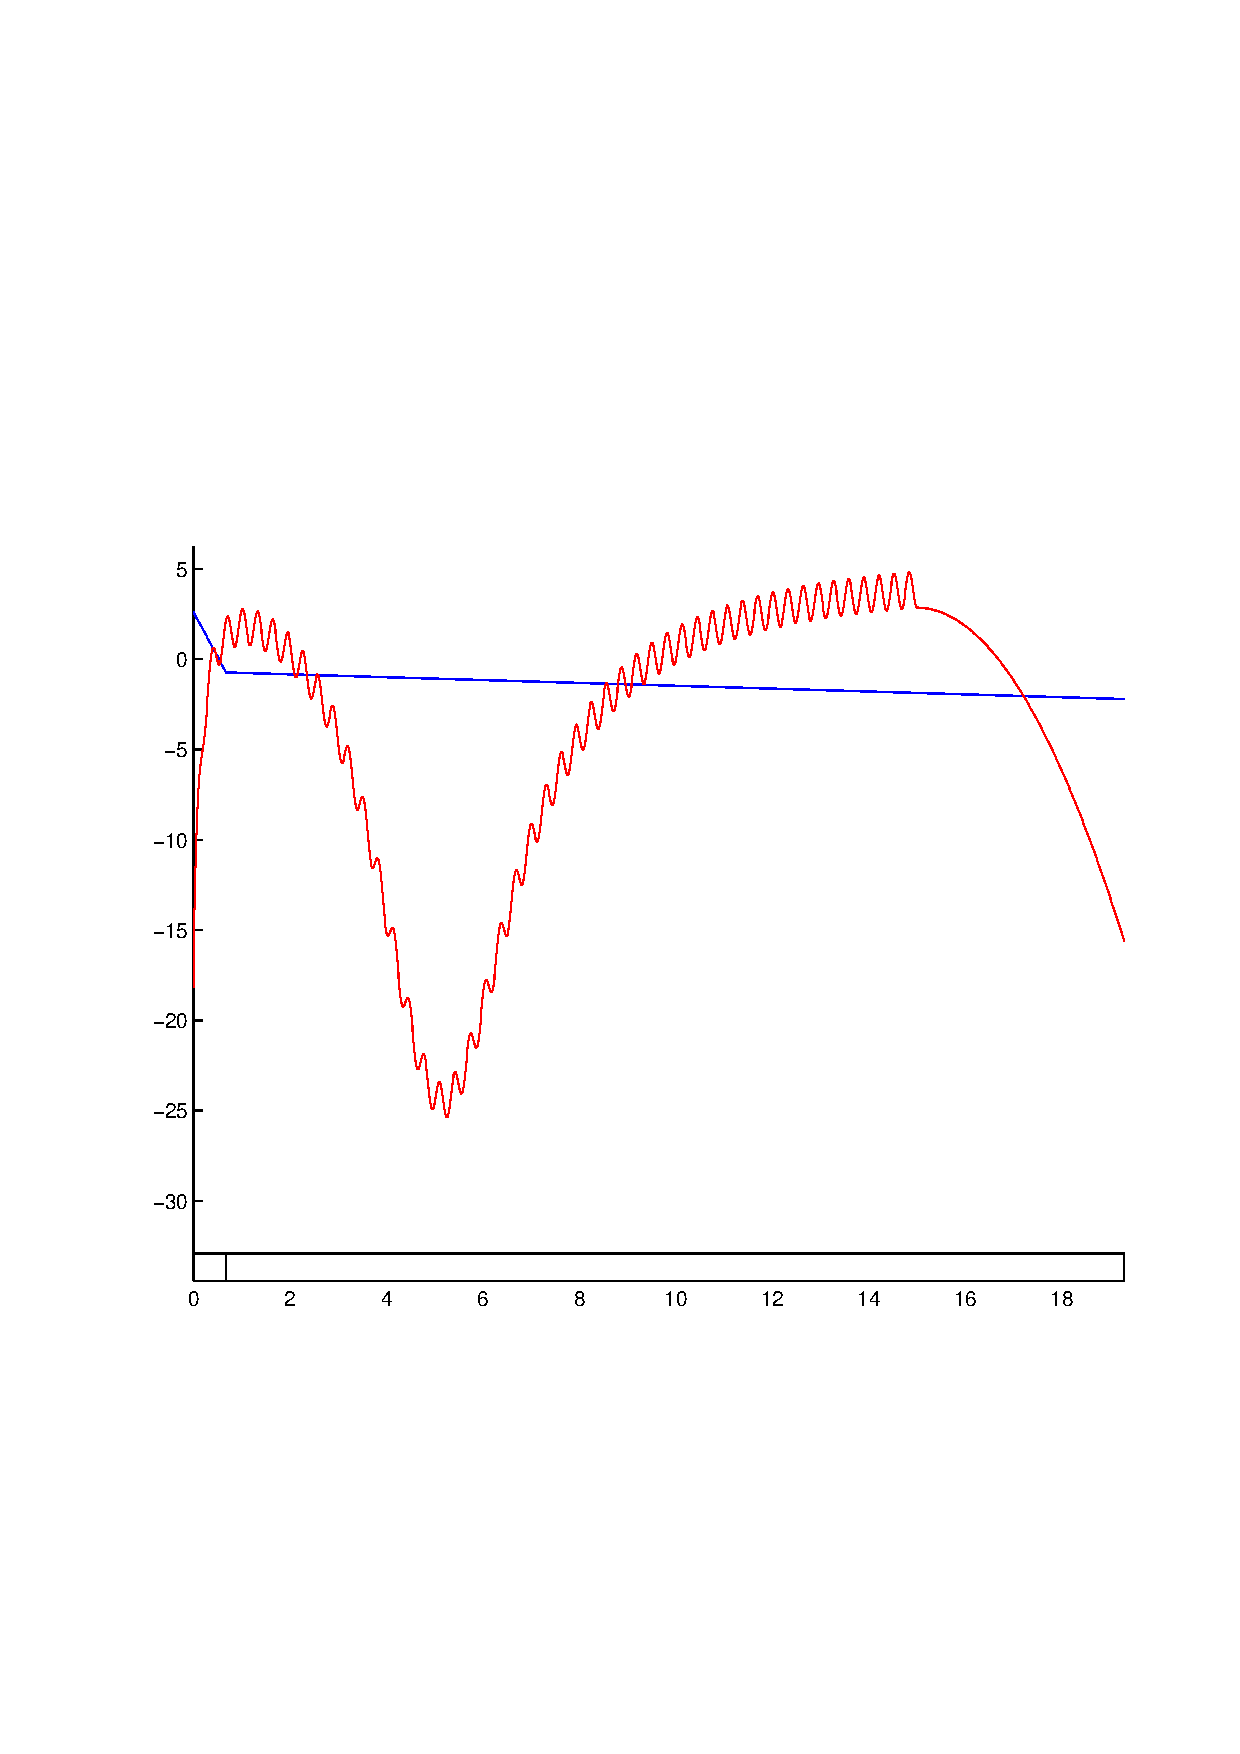
\includegraphics[width=0.3\textwidth]{Figure1}
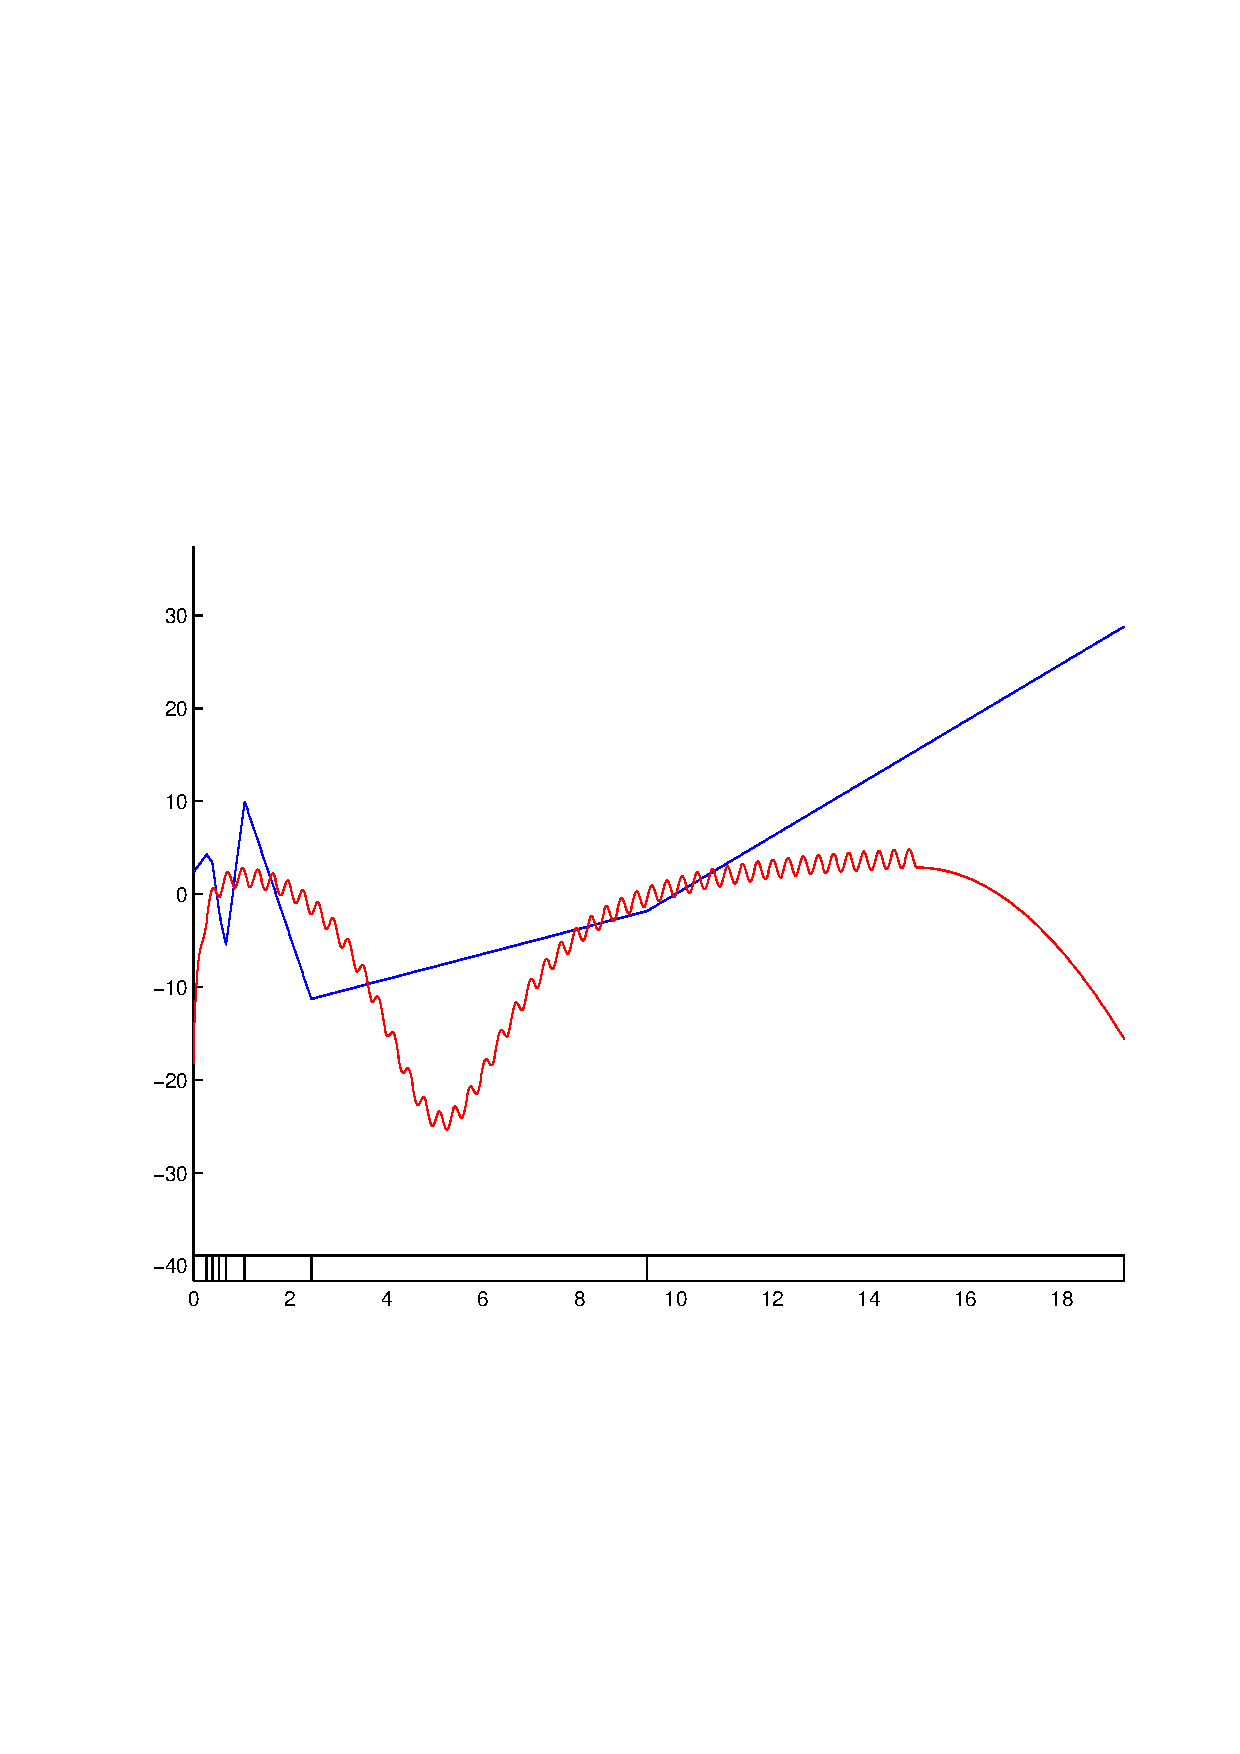
\includegraphics[width=0.3\textwidth]{Figure3}
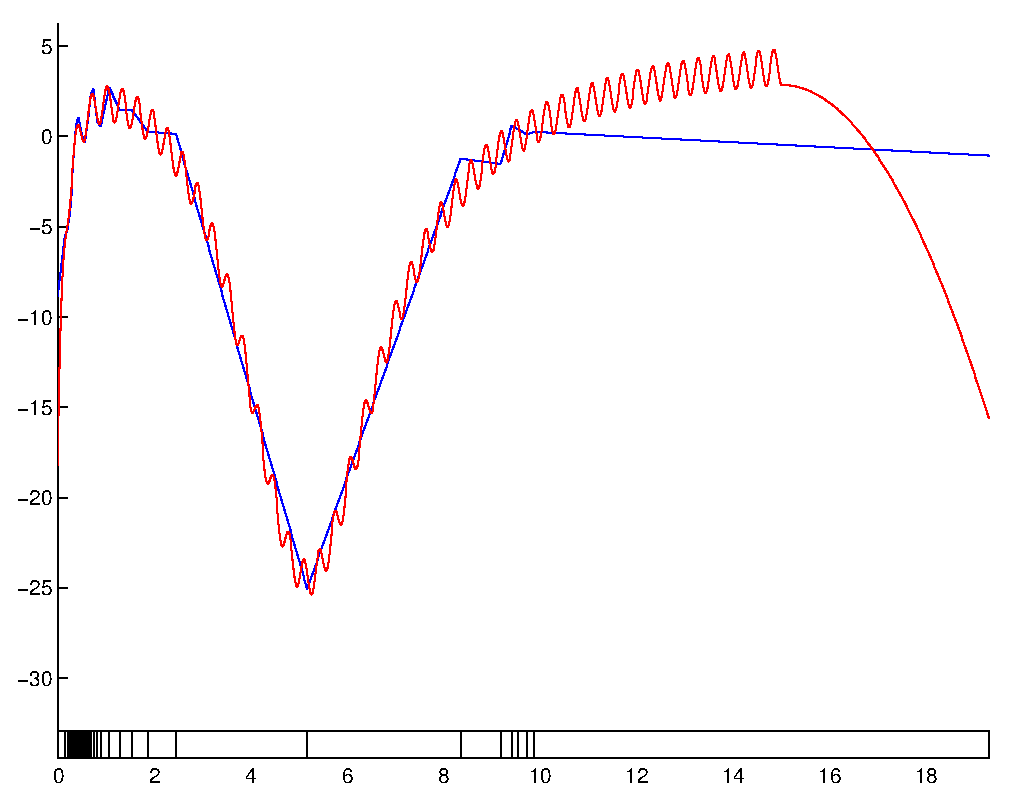
\includegraphics[width=0.3\textwidth]{Figure5}
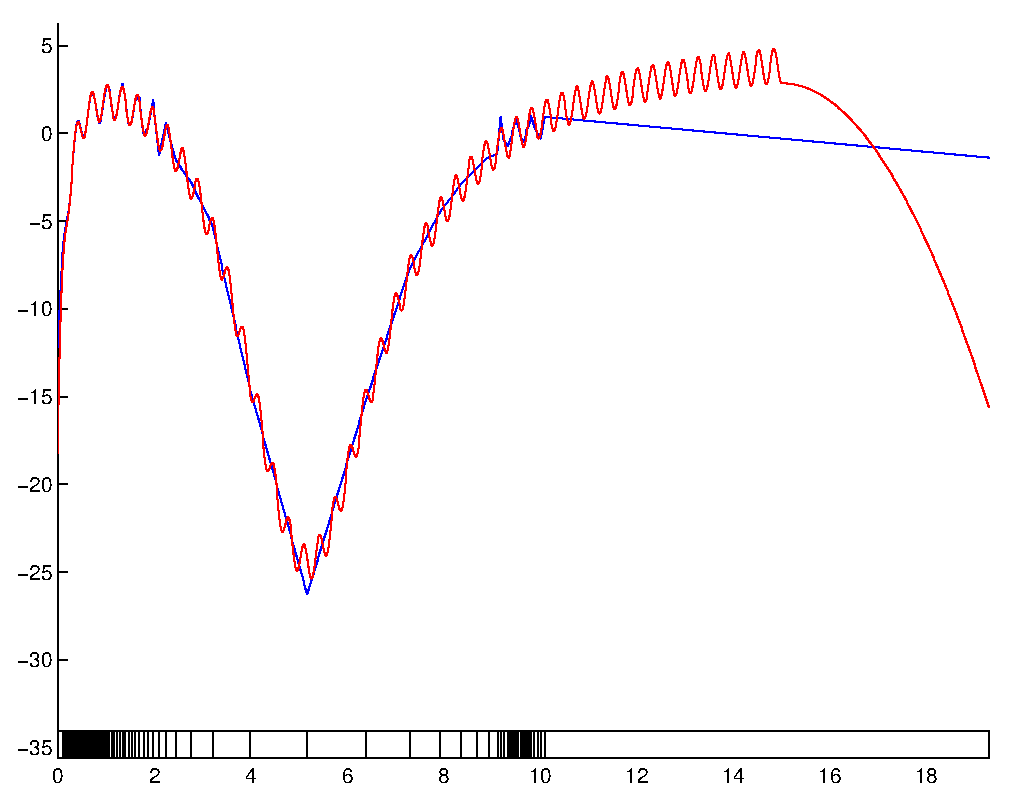
\includegraphics[width=0.3\textwidth]{Figure7}
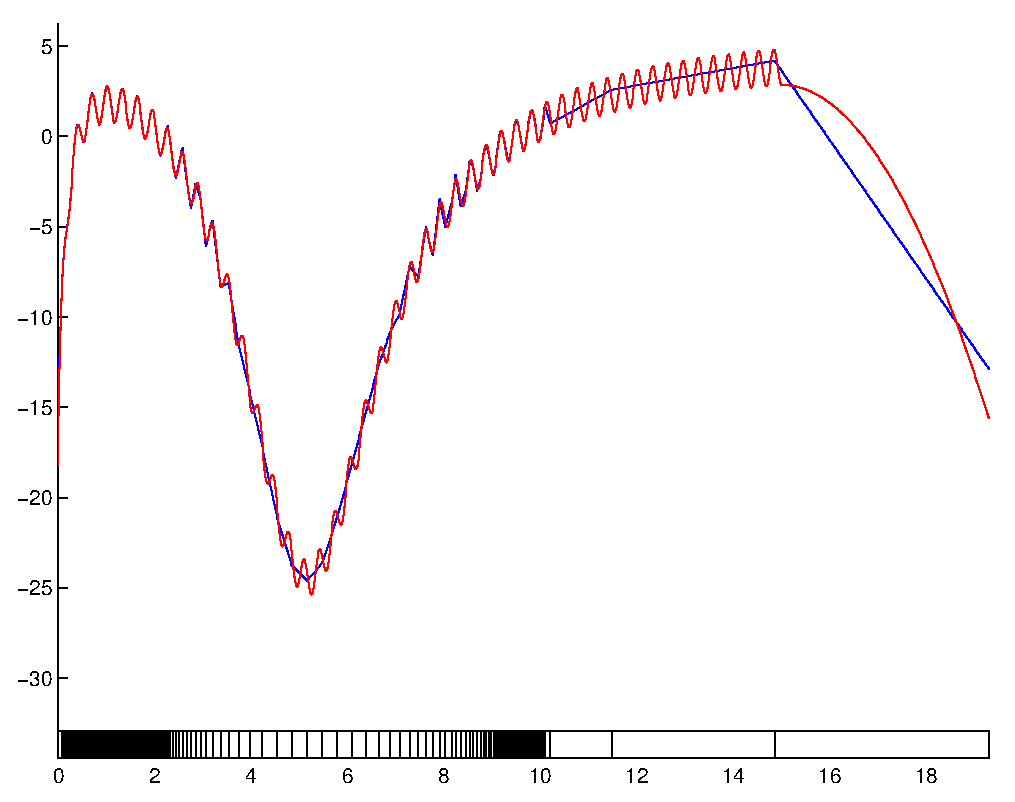
\includegraphics[width=0.3\textwidth]{Figure9}
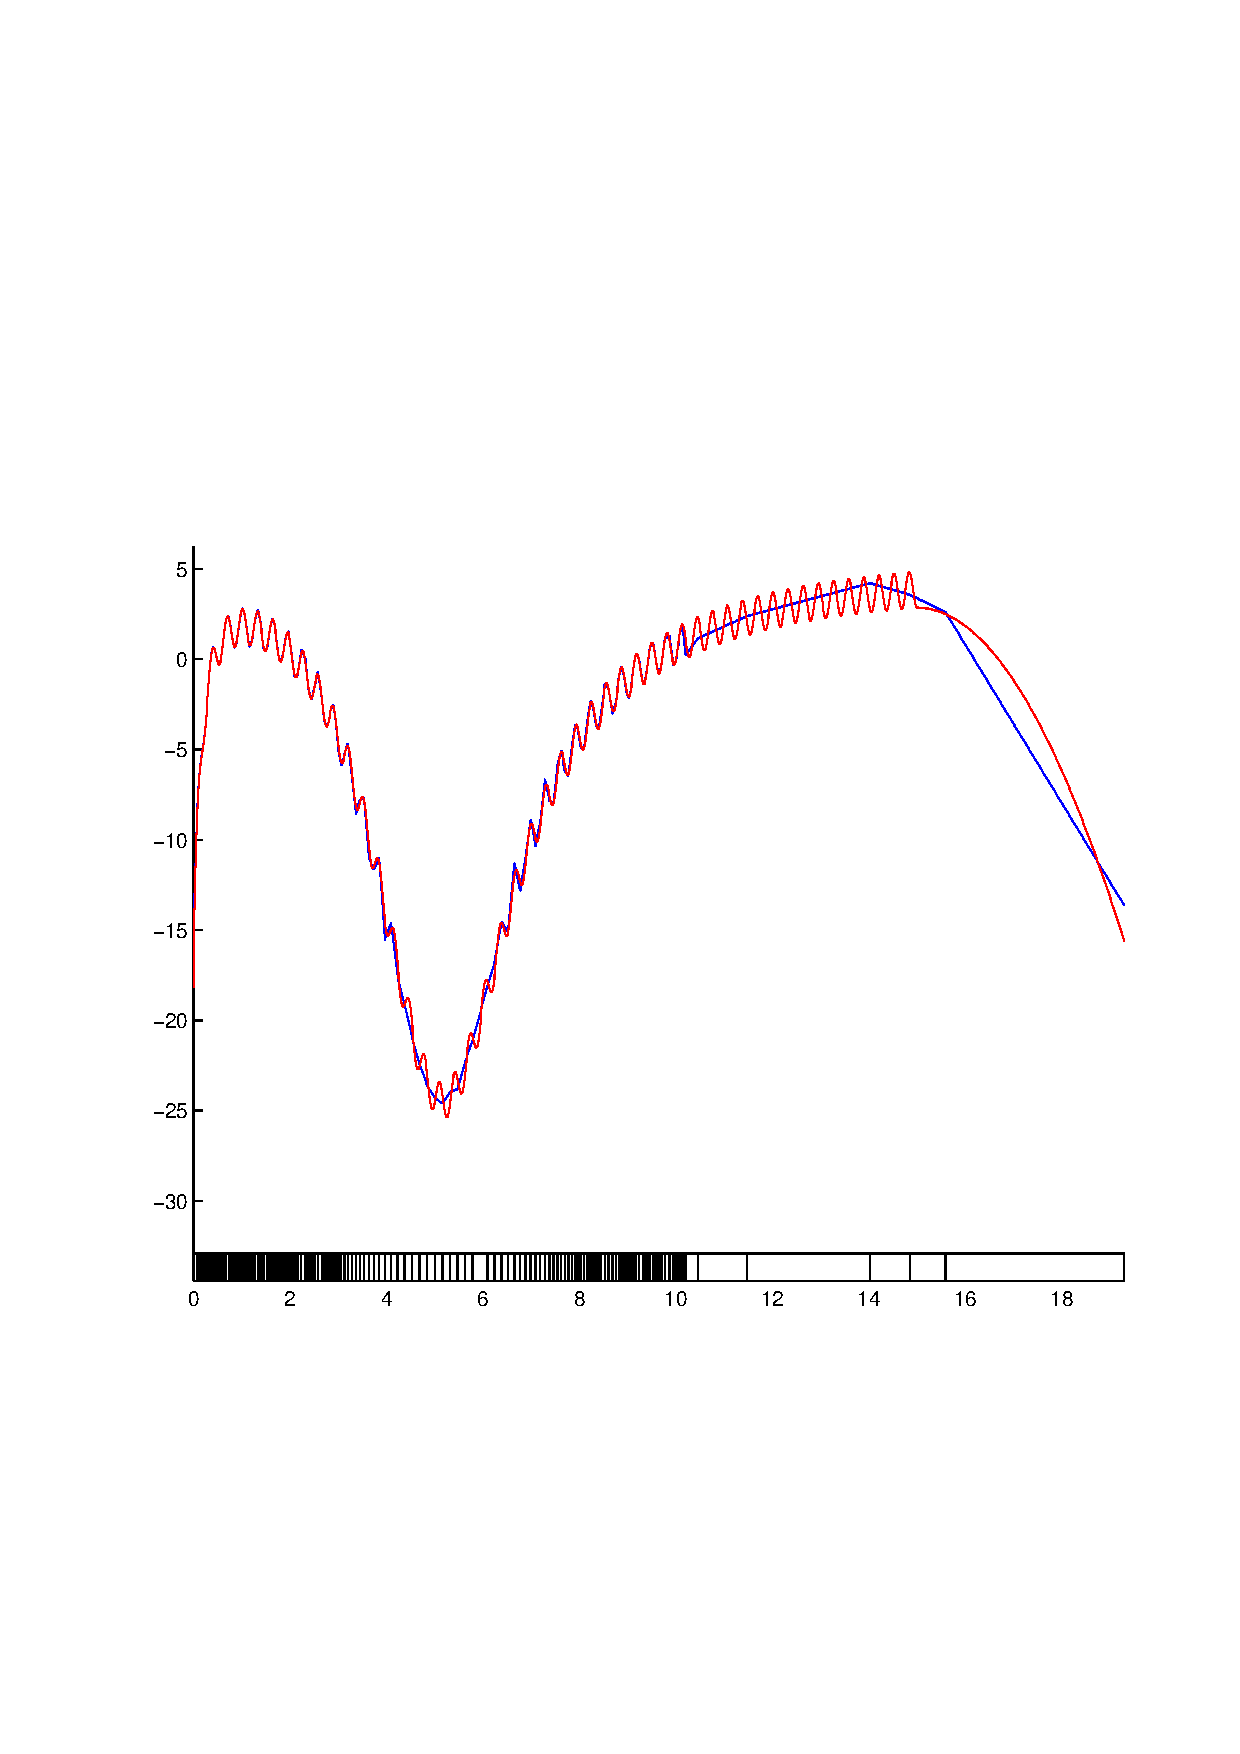
\includegraphics[width=0.3\textwidth]{Figure11} 
\end{center}
\caption{First preliminary numerical experiments indicating the successful recovery by an adaptive algorithm based on \eqref{fdproxy} of a potential function $a$ in a first order model of the type \eqref{fdgradientflow}. The potential $a$ to be recovered is displayed in red color and it's the strongly oscillating function. The blue function is the piecewise linear approximant computed at each successive iteration after adaptation of the underlying mesh, scketched on the bottom of the figures.}\label{firstnum}
\end{figure}

Despite the highly oscillatory nature of the parameter function $a$, the algorithm performs an excellent approximation, providing also a sort of "numerical homogenization" in those locations of the positive real line, where not enough data are provided by the evolution.
\section{Appendix}

\subsection{Technical lemmas for the mean-field limit}\label{ap1}

The following preliminary result tells us that solutions to system \eqref{eq:discrdyn} are also solutions to systems \eqref{eq:contdyn}, whenever conveniently rewritten.

\begin{proposition}\label{p-rewritten}
Let $N \in \N$ be given. Let $(x^N_1, \ldots, x^N_N):[0,T] \rightarrow \R^{dN}$ be the solution of \eqref{eq:discrdyn} with initial datum $x^{N}_0 \in \R^{dN}$. Then the empirical measure $\mu^N:[0,T] \rightarrow \PP(\R^d)$ defined as in \eqref{eq:empmeas} is a solution of \eqref{eq:contdyn} with initial datum $\mu_{0}= \mu^N(0) \in \PC(\R^d)$.
\end{proposition}
\begin{proof}
It can be easily proved by arguing exactly as in \cite[Lemma 4.3]{MFOC}.
\end{proof}

 We are able to state several basic estimates that shall be useful towards an existence and uniqueness result for the solutions of system \eqref{eq:discrdyn}.

\begin{lemma}\label{p-estkernel}
Let $a\in X$ and $\mu \in \PP(\R^d)$. Then for all $y \in \R^d$ the following hold:
\begin{align*}
|(F[a] * \mu)(y)| \leq \|a\|_{L_{\infty}(\R_+)}\left( | y | + \int_{\R^d} | x | d\mu(x) \right).
\end{align*}
\end{lemma}
\begin{proof}
Trivially follows from $a \in L_{\infty}(\R_+)$.
\end{proof}

\begin{lemma}\label{p-Floclip}
If $a\in X$ then $F[a] \in \Lip_\loc(\R^d)$.
\end{lemma}
\begin{proof}
For any compact set $K \subset \R^d$ and for every $x,y \in K$ it holds
\begin{align*}
|F[a](x) - F[a](y)| &= |a(|x|)x - a(|y|)y| \\
&\leq |a(|x|)| |x-y| + |a(|x|) - a(|y|)| |y| \\
&\leq (|a(|x|)| + \Lip_K(a) |y|) |x-y|,
\end{align*}
and since $a \in L_{\infty}(\R_+)$ and $y \in K$, it follows that $F[a]$ is locally Lipschitz with Lipschitz constant depending only on $a$ and $K$.
\end{proof}

\begin{lemma}\label{p-Fmuloclip}
If $a\in X$ and $\mu \in \mathcal{P}_c(\R^d)$ then $F[a]*\mu \in \Lip_{\loc}(\R^d)$.
\end{lemma}
\begin{proof}
For any compact set $K \subset \R^d$ and for every $x,y \in K$ it holds
\begin{align*}
|(F[a]*\mu)(x) - (F[a]*\mu)(y)| &= \left|\int_{\R^d}a(|x-z|)(x-z)d\mu(z) - \int_{\R^d}a(|y-z|)(y-z)d\mu(z)\right| \\
&\leq \int_{\R^d}|a(|x-z|)-a(|y-z|)|x-z|d\mu(z)\\
&\quad+ \int_{\R^d}a(|y-z|)|x-y|d\mu(z) \\
&\leq \Lip_{\widehat{K}}(a)|x-y| \int_{\R^d}|x-z|d\mu(z) + \|a\|_{L_{\infty}(\R_+)}|x-y| \\
&\leq \left(\Lip_{\widehat{K}}(a)(|x| + 1)+ \|a\|_{L_{\infty}(\R_+)}\right)|x-y| \\
& \leq \left(C\Lip_{\widehat{K}}(a) + \|a\|_{L_{\infty}(\R_+)} \right)|x-y|,
\end{align*}
where $C$ is a constant depending on $K$, and $\widehat{K}$ is a compact set containing both $K$ and $\supp(\mu)$.
\end{proof}



\begin{proposition}
If $a \in X$ then system \eqref{eq:discrdyn} admits a unique global solution in $[0,T]$ for every initial datum $x^{N}_0 \in \R^{dN}$.
\end{proposition}
\begin{proof}
Rewriting system \eqref{eq:discrdyn} in the form of \eqref{eq:discr1}, from Lemma \ref{p-Fmuloclip} follows trivially that the function $G:\R^{dN} \rightarrow \R^{dN}$ defined for every $(x_1, \ldots, x_N)\in \R^{dN}$ as
\begin{align*}
G(x_1, \ldots, x_N) = ((F[a]*\mu^N)(x_1),\ldots,(F[a]*\mu^N)(x_N)),
\end{align*}
where $\mu^N$ is the empirical measure given by \eqref{eq:empmeas}, satisfies $G \in \Lip_\loc(\R^{dN})$. The Cauchy-Lipschitz Theorem for ODE systems then yields the desired result.
\end{proof}

Variants of the following result are \cite[Lemma 6.7]{MFOC} and \cite[Lemma 4.7]{CanCarRos10}

\begin{lemma}\label{p-lipkernel}
Let $a \in X$ and let $\mu:[0,T] \rightarrow \mathcal{P}_c(\R^d)$ and $\nu: [0,T] \to \PP(\R^d)$ be two continuous maps with respect to $\W_1$ satisfying
\begin{align}\label{eq:bsupp}
\supp(\mu(t)) \cup \supp(\nu(t)) \subseteq B(0,R),
\end{align}
for every $t \in [0,T]$, for some $R > 0$. Then for every $r > 0$ there exists a constant $L_{a,r,R}$ such that
\begin{align}\label{eq:inftynormW1}
\|F[a] * \mu(t) - F[a] * \nu(t)\|_{L_{\infty}(B(0,r))} \leq L_{a,r,R} \W_1(\mu(t),\nu(t))
\end{align}
for every $t \in [0,T]$.
\end{lemma}
\begin{proof}
Fix $t \in [0,T]$ and take $\pi \in \Gamma_o(\mu(t),\nu(t))$. Since the marginals of $\pi$ are by definition $\mu(t)$ and $\nu(t)$, it follows
\begin{align*}
F[a] * \mu(t)(x) - F[a] * \nu(t)(x) &= \int_{B(0,R)} F[a](x-y) d\mu(t)(y) - \int_{B(0,R)} F[a](x-z) d\nu(t)(z)  \\
&= \int_{B(0,R)^2} \left(F[a](x-y) - F[a](x-z)\right) d\pi(y,z)
\end{align*}
By using Lemma \ref{p-Floclip} and the hypothesis \eqref{eq:bsupp}, we have
\begin{align*}
\|F[a] * \mu(t) - F[a] * \nu(t)\|_{L_{\infty}(B(0,r))} &\leq \esssup_{x \in B(0,r)} \int_{B(0,R)^2} \left|F[a](x-y) - F[a](x-z)\right| d\pi(y,z) \\
&\leq \Lip_{B(0,R+r)}(F[a]) \int_{B(0,R)^2} |y - z| d\pi(y,z) \\
&= \Lip_{B(0,R+r)}(F[a]) \W_1(\mu(t),\nu(t)),
\end{align*}
hence \eqref{eq:inftynormW1} holds with $L_{a,r,R} = \Lip_{B(0,R+r)}(F[a])$.
\end{proof}


\subsection{Proof of Proposition \ref{pr:exist}}\label{ap2}

Notice that for every $N \in \N$, by Proposition \ref{p-rewritten}, $\mu^N$ is the unique solution of \eqref{eq:contdyn} with initial datum $\mu^N_0$. We start by fixing $N \in \N$ and estimating the growth of $|x_i^N(t)|^2$ for $i = 1, \ldots, N$. By using Lemma \ref{p-estkernel}, we have
\begin{align*}
\frac{1}{2}\frac{d}{dt} |x_i^N(t)|^2 & \leq \dot{x}_i^N(t) \cdot x_i^N(t) \\
& \leq \left|(F[a]*\mu^N(t))(x_i(t))\right| |x_i^N(t)| \\
& \leq \|a\|_{L_{\infty}(\R_+)}\left( |x_i^N(t)| + \frac{1}{N} \sum^N_{j = 1}|x_j^N(t)| \right) |x_i^N(t)| \\
& \leq 2 \|a\|_{L_{\infty}(\R_+)}\max_{j = 1, \ldots, N} |x_j^N(t)| |x_i^N(t)| \\
& \leq 2 \|a\|_{L_{\infty}(\R_+)}\max_{j = 1, \ldots, N} |x_j^N(t)|^2.
\end{align*}
If we denote by $q(t) := \max_{j = 1, \ldots, N} |x_j^N(t)|^2$, then the Lipschitz continuity of $q$ implies that $q$ is a.e. differentiable. Stampacchia's Lemma \cite[Chapter 2, Lemma A.4]{Kin-Sta} ensures that for a.e. $t \in [0,T]$ there exists $k = 1, \ldots, N$ such that
\begin{align*}
\dot{q}(t) = \frac{d}{dt} |x_k^N(t)|^2 \leq 4 \|a\|_{L_{\infty}(\R_+)} q(t).
\end{align*}
Hence, Gronwall's Lemma and the hypothesis $x^{N}_{0,i} \in \supp(\mu_0) + \overline{B(0,1)}$ for every $N \in \N$ and $i = 1, \ldots, N$, imply that
\begin{align*}
q(t) \leq q(0) e^{4 \|a\|_{L_{\infty}(\R_+)} t} \leq C_0 e^{4 \|a\|_{L_{\infty}(\R_+)} t} \text{ for a.e. } t \in [0,T],
\end{align*}
for some uniform constant $C_0$ depending only on $\mu_0$. Therefore, the trajectory $\mu^N(\cdot)$ is bounded uniformly in $N$ in a ball $B(0,R) \subset \R^d$, where
\begin{align}\label{Rest}
R =  \sqrt{C_0} e^{2 \|a\|_{L_{\infty}(\R_+)} T}.
\end{align}
This, in turn, implies that $\mu^N(\cdot)$ is Lipschitz continuous with Lipschitz constant uniform in $N$, since by the fact that $|x^N_i(t)| \leq R$ for a.e. $t \in [0,T]$, for all $N \in N$ and $i = 1, \ldots, N$, and Lemma \ref{p-estkernel} follows
\begin{align*}
|\dot{x}^N_i(t)| &= |(F[a]*\mu^N(t))(x^N_i(t))| \\
&\leq \|a\|_{L_{\infty}(\R_+)} \left( |x^N_i(t)| + \frac{1}{N}\sum^N_{j = 1}|x^N_j(t)|\right) \\
&\leq 2R\|a\|_{L_{\infty}(\R_+)}.
\end{align*}
We have thus found a sequence $(\mu^N)_{N \in \N} \subset \mathcal{C}^0([0,T],\mathcal{P}_1(B(0,R)))$ for which the following holds:
\begin{itemize}
\item $(\mu^N)_{N \in \N}$ is equicontinuous and closed, because of the uniform Lipschitz constant $2R\|a\|_{L_{\infty}(\R_+)}$;
\item for every $t \in [0,T]$, the sequence $(\mu^N(t))_{N \in \N}$ is relatively compact in $\mathcal{P}_1(B(0,R))$. This holds because $(\mu^N(t))_{N \in \N}$ is a tight sequence, since $B(0,R)$ is compact, and hence relatively compact due to Prokhorov's Theorem.
\end{itemize}
Therefore, we can apply the Ascoli-Arzel\'{a} Theorem for functions with values in a metric space (see for instance, \cite[Chapter 7, Theorem 18]{KelleyTop}) to infer the existence of a subsequence $(\mu^{N_k})_{k \in \N}$ of $(\mu^N)_{N \in \N}$ such that
\begin{align}\label{eq:unifconv}
\lim_{k \rightarrow \infty}\W_1(\mu^{N_k}(t),\mu(t)) = 0 \quad \text{ uniformly for a.e. } t \in [0,T],
\end{align}
for some $\mu \in \mathcal{C}^0([0,T],\mathcal{P}_1(B(0,R)))$ with Lipschitz constant bounded by $2R\|a\|_{L_{\infty}(\R_+)}$. The hypothesis $\lim_{N\rightarrow\infty}\W_1(\mu^N_0,\mu_0) = 0$ now obviously implies $\mu(0) = \mu_0$.

We are now left with verifying that this curve $\mu$ is a solution of \eqref{eq:contdyn}. For all $t \in [0,T]$ and for all $\varphi \in \mathcal{C}^1_c(\R^d;\R)$, since it holds
\begin{align*}
\frac{d}{dt}\langle \varphi, \mu^N(t) \rangle = \frac{1}{N}\frac{d}{dt} \sum^N_{i = 1} \varphi(x^N_i(t)) = \frac{1}{N} \sum^N_{i = 1} \nabla\varphi(x^N_i(t)) \cdot \dot{x}_i^N(t),
\end{align*}
by directly applying the substitution $\dot{x}_i^N(t) = (F[a]*\mu^N(t))(x^N_i(t))$, we have
\begin{align*}
\langle \varphi, \mu^N(t) - \mu^N(0) \rangle = \int^t_0 \left[ \int_{\R^d}\nabla \varphi(x) \cdot (F[a]*\mu^N(s))(x) d\mu^N(s)(x) \right] ds.
\end{align*}
By Lemma \ref{p-lipkernel}, the inequality \eqref{eq:unifconv}, and the compact support of $\varphi \in \mathcal{C}^1_c(\R^d;\R)$, follows
\begin{align*}
\lim_{N \rightarrow \infty} \|\nabla\varphi \cdot (F[a]*\mu^N(t) - F[a]*\mu(t))\|_{L_{\infty}(\R^d)} = 0 \quad \text{ uniformly for a.e. } t \in [0,T].
\end{align*}
If we denote with $\mathcal L_1\llcorner_{[0,t]}$ the Lebesgue measure on the time interval $[0,t]$, since the product measures $\frac{1}{t} \mu^{N}(s) \times \mathcal L_1\llcorner_{[0,t]}$ converge in $\mathcal P_1([0,t] \times \mathbb R^{d})$ to $\frac{1}{t} \mu(s) \times \mathcal L_1\llcorner_{[0,t]}$, we finally get from the dominated convergence theorem that
\begin{align*}
\lim_{N \to \infty} \int_0^{t} \int_{\mathbb R^{d}} \nabla \phi(x) \cdot (F[a]*&\mu^N(s))(x) d\mu^N(s)(x) ds \\
&=  \int_0^{t} \int_{\mathbb R^{d}} \nabla \phi(x) \cdot (F[a]*\mu(s))(x) d \mu(s)(x) ds,
\end{align*}
which proves that $\mu$ is a solution of \eqref{eq:contdyn} with initial datum $\mu_0$.


\subsection{Existence and uniqueness of solutions for  \eqref{eq:transpdyn}}\label{ap3}

For the reader's convenience we start by briefly recalling some general, well-known results about solutions to Carath{\'e}odory differential equations. We fix a domain $\Omega \subset \R^d$, a Carath{\'e}odory function $g\colon[0,T]\times \Omega \to \R^d$, and $0<\tau \le T$. A function $y\colon [0,\tau]\to \Omega$ is called a solution of the Carath{\'e}odory differential equation
\begin{equation}\label{cara}
\dot y(t)=g(t, y(t))
\end{equation}
on $[0,\tau]$ if and only if $y$ is absolutely continuous and \eqref{cara} is satisfied a.e.\ in $[0,\tau]$.
The following existence result holds.
%\begin{theorem}\label{cara2}
%Consider an interval $[0,T]$ on the real line and a domain $\Omega \subset \R^n$, for $n\ge 1$. Let $g\colon[0,T]\times \Omega \to \R^n$ be a Carath{\'e}odory function for which there exists a function $m \in L_1((0,T))$ such that
%$$
%|g(t,y)|\le m(t)
%$$
%for a.e.\ $t \in [0,T]$ and every $y \in \Omega$. Then, given $y_0 \in \Omega$, there exists $0<\tau \le T$ and a solution $y(t)$ of \eqref{cara} on $[0,\tau]$ satisfying $y(0)=y_0$. 
%
%If in addition there exists a function $l \in L_1((0,T))$ such that
%\begin{equation}\label{cara3}
%|g(t,y_1)-g(t, y_2)|\le l(t)|y_1-y_2|
%\end{equation}
%for a.e.\ $t \in [0,T]$ and every $y_1$, $y_2 \in \Omega$, the solution is uniquely determined on $[0,\tau]$ by the initial condition $y_0$.
%\end{theorem}
%
%\begin{proof}
%See, for instance, \cite[Chapter 1, Theorems 1 and 2]{Fil}.
%\end{proof}
%
%What follows is a generalization of the global existence theorem and of a Gronwall-type estimate on the solutions to this setting.

\begin{theorem}\label{cara-global}
Fix $T > 0$ and $y_0 \in \R^d$. Suppose that there exists a compact subset $\Omega$ of $\R^d$ such that $y_0 \in \textup{int}(\Omega)$ and there exists $m_{\Omega} \in L_1([0,T])$ for which it holds
%Consider an interval $[0,T]$ on the real line, a compact subset $K$ of $\R^n$, and a Carath{\'e}odory function $g\colon[0,T]\times \R^n \to \R^n$. If there exists a function $m \in L_1((0,T))$ such that
\begin{align}\label{l1}
|g(t,y)|\le m_{\Omega}(t),
\end{align}
for a.e.\ $t \in [0,T]$ and for all $y \in \Omega$. Then there exists a $\tau > 0$ and a solution $y(t)$ of \eqref{cara} defined on the interval $[0,\tau]$ which satisfies $y(0)=y_0$. If there exists $C > 0$ such that the function $g$ also satisfies the condition
\begin{align}\label{ttz}
|g(t,y)|\le C(1+|y|),
\end{align}
for a.e.\ $t \in [0,T]$ and every $y \in \Omega$, and it holds $B(0,R) \subseteq \Omega$, for $R > |y_0| + CT e^{CT}$, then the local solution $y(t)$ of \eqref{cara} which satisfies $y(0)=y_0$ can be extended to the whole interval $[0,T]$. Moreover, for every $t \in [0,T]$, any solution satisfies
\begin{equation}\label{gron}
|y(t)|\le \Big(|y_0|+ Ct\Big) \,e^{Ct}.
\end{equation}
%If in addition, for every relatively compact open subset $\Omega \subset \R^d$ there exists a constant $L_{\Omega}$ for which it holds
%\begin{align}\label{cara3}
%|g(t,y_1)-g(t, y_2)|\le L_{\Omega}|y_1-y_2|,
%\end{align}
%for a.e.\ $t \in [0,T]$ and every $y_1$, $y_2 \in \Omega$, then the solution is uniquely determined on $[0,T]$ by the initial condition $y_0$.
\end{theorem}

\begin{proof}
%Set $\rho:= (|y_0|+CT) \,e^{CT}$ and
Since $y_0 \in \textup{int}(\Omega)$, we can consider a ball $B(y_0,r) \subset \Omega$. The classical result \cite[Chapter 1, Theorem 1]{Fil} and \eqref{l1} yield the existence of a local solution defined on an interval $[0,\tau]$ and taking values in $B(y_0,r)$.

If \eqref{ttz} holds, any solution of \eqref{cara} with initial datum $y_0$ satisfies
$$
|y(t)|\le |y_0|+ Ct+C\int_0^t |y(s)|\,ds
$$
for every $t \in [0,\tau]$, therefore \eqref{gron} follows from Gronwall's inequality. In particular the graph of a solution $y(t)$ cannot reach the boundary of $[0,T]\times B(0,|y_0|+CTe^{CT})$ unless $\tau=T$, therefore the continuation of the local solution to a global one on $[0,T]$ follows, for instance, from \cite[Chapter 1, Theorem 4]{Fil}.
%Finally, if \eqref{cara3} holds, uniqueness of the global solution follows from \cite[Chapter 1, Theorem 2]{Fil}.
\end{proof}

Gronwall's inequality easily gives us the following results on continuous dependence on the initial data.

\begin{lemma}\label{le:uniquecara}
Let $g_1$ and $g_2\colon[0,T]\times \R^n \to \R^n$ be Carath{\'e}odory functions both satisfying \eqref{ttz} for the same  constant $C > 0$. Let $r>0$ and define 
\begin{align*}
\rho_{r, C, T}:=\Big(r+ CT\Big) \,e^{CT}\,.
\end{align*}
Assume in addition that there exists a constant $L > 0$ satisfying
\begin{align*}
|g_1(t, y_1)-g_1(t, y_2)|\le L|y_1-y_2|
\end{align*}
for every $t \in [0, T]$ and every $y_1$, $y_2$ such that $|y_i|\le \rho_{r, C, T}$, $i=1,2$.
Then, if $\dot y_1(t)=g_1(t, y_1(t))$, $\dot y_2(t)=g_2(t, y_2(t))$, $|y_1(0)|\le r$ and $|y_2(0)|\le r$, one has
\begin{equation}\label{gronvalla}
|y_1(t)-y_2(t)|\le e^{Lt}\left(|y_1(0)-y_2(0)|+\int_0^t \|g_1(s, \cdot)-g_2(s, \cdot)\|_{L_\infty(B(0, \rho_{r, C, T}))} \,ds \right)
\end{equation}
for every $t \in [0, T]$.
\end{lemma}
\begin{proof}
We can bound $|y_1(t) - y_2(t)|$ from above as follows:
\begin{align*}
|y_1(t) - y_2(t)| &\leq |y_1(0) - y_2(0)| + \int^t_0 |\dot{y}_1(s) - \dot{y}_2(s)| ds \\
&= |y_1(0) - y_2(0)| \\
& \quad + \int^t_0 |g_1(s, y_1(s)) - g_1(s, y_2(s)) + g_1(s, y_2(s)) - g_2(s, y_2(s))| ds \\
& \leq |y_1(0) - y_2(0)| + \int_0^t \|g_1(s, \cdot)-g_2(s, \cdot)\|_{L_\infty(B(0, \rho_{r, C, T}))} \,ds \\
& \quad  + L \int^t_0|y_1(s) - y_2(s)| ds.
\end{align*}
Since the function $\alpha(t) = |y_1(0) - y_2(0)| + \int_0^t \|g_1(s, \cdot)-g_2(s, \cdot)\|_{L_\infty(B(0, \rho_{r, C, T}))} \,ds$ is increasing, an application of Gronwall's inequality gives \eqref{gronvalla}, as desired.
\end{proof}


\begin{proposition}
Fix $T > 0$, $a \in X$, $\mu_0 \in \mathcal{P}_c(\R^d)$, $\xi_0 \in \R^d$ and let $R > 0$ be given by Proposition \ref{pr:exist} from the choice of $T, a$ and $\mu_0$. For every map $\mu:[0,T] \rightarrow \PP(\R^d)$ which is continuous with respect to $\W_1$ such that
\begin{align*}
\supp(\mu(t)) \subseteq B(0,R) \quad \text{ for every } t \in [0,T],
\end{align*}
there exists a unique solution of system \eqref{eq:transpdyn} with initial value $\mu_0$ defined on the whole interval $[0,T]$.
\end{proposition}
\begin{proof}
By Lemma \ref{p-estkernel} follows that, for any compact set $K \subset \R^d$ containing $\xi_0$, there exists a function $m_K \in L_1([0,T])$ for which the function $g(t,y)=(F[a]\ast\mu(t))(y)$ satisfies \eqref{l1}. Moreover, for fixed $t$ this function is locally Lipschitz continuous, as follows from Lemma \ref{p-Fmuloclip}, thus $g(t,y)=(F[a]\ast\mu(t))(y)$ is a Carath\'eodory function.

%Notice that $a \in L_{\infty}(\R_+)$ trivially implies that of $F[a] \in L_{\infty}_{\loc}(\R^d)$. This, together with Lemma \ref{p-estkernel} and the hypothesis that $\supp(\mu(t)) \subseteq B(0,R)$ for all $t \in [0,T]$, yields $F[a]\ast\mu(t)\in L_{\infty}(\R_+)$ uniformly in $t$, hence \eqref{l1} holds. 
		
From the hypothesis that the support of $\mu$ is contained in $B(0,R)$ and Lemma \ref{p-estkernel}, follows the existence of a constant $C$ depending on $T,a$ and $\mu_0$ such that
\begin{align*}
|(F[a]*\mu(t))(y)| &\leq C(1+|y|)
\end{align*}
holds for every $y \in \R^d$ and for every $t \in [0,T]$. Hence $F[a]*\mu(t)$ is sublinear and \eqref{ttz} holds. By considering a sufficiently large compact set $K$ containing $\xi_0$, Theorem \ref{cara-global} guarantees the existence of a solution of system \eqref{eq:transpdyn} defined on $[0,T]$.

To establish uniqueness notice that, from Lemma \ref{p-Floclip}, for every compact subset $K \in \R^d$ and any $x,y \in K$, it holds
\begin{align}
\begin{split}\label{eq:uniquecara}
|(F[a]*\mu(t))(x) - (F[a]*\mu(t))(y)| &\leq \left| \int_{\R^d}F[a](x-z)d\mu(t)(z) - \int_{\R^d}F[a](y-z)d\mu(t)(z)\right| \\
&\leq \int_{\R^d} \left|F[a](x-z) - F[a](y-z)\right|d\mu(t)(z) \\
&\leq \Lip_{\widehat{K}}(F[a]) |x-y|,
\end{split}\end{align}
where $\widehat{K}$ is a compact set containing both $K$ and $B(0,R)$. Hence, uniqueness follows from \eqref{eq:uniquecara} and Lemma \ref{le:uniquecara} by taking $g_1 = g_2$, $y_1(0) = y_2(0)$ and $r = |y_1(0)|$.
\end{proof}

\subsection{Continuous dependence on the initial data}\label{ap4}

The following Lemma and \eqref{gronvalla} are the main ingredients of the proof of Theorem \ref{uniq} on continuous dependance on initial data.

\begin{lemma}\label{primstim}
Let $\mathcal{T}_1$ and $\mathcal{T}_2 \colon \R^n \to \R^n$ be two bounded Borel measurable functions. Then, for every $\mu \in \PP(\R^n)$ one has
\begin{align*}
\W_1((\mathcal{T}_1)_{\#}\mu, (\mathcal{T}_2)_{\#} \mu) \le \|\mathcal{T}_1-\mathcal{T}_2\|_{L_\infty({\rm supp}\,\mu)}.
\end{align*}
If in addition $\mathcal{T}_1$ is locally Lipschitz continuous, and $\mu$, $\nu \in \PP(\R^n)$ are both compactly supported on a ball $B(0,r)$ of $\R^n$, then
\begin{align*}
\W_1((\mathcal{T}_1)_{\#} \mu, (\mathcal{T}_1)_{\#} \nu) \le \Lip_{B(0,r)}(E_1) \W_1(\mu, \nu).
\end{align*}
\end{lemma}

\begin{proof}
See \cite[Lemma 3.11]{CanCarRos10} and \cite[Lemma 3.13]{CanCarRos10}.
\end{proof}

We can now prove Theorem \ref{uniq}.

\begin{proof}[Proof of Theorem \ref{uniq}]
Let  ${\mathcal T}^\mu_t$ and ${\mathcal T}^\nu_t$ be the flow maps associated to system \eqref{eq:transpdyn} with measure $\mu$ and $\nu$, respectively.
By \eqref{eq:fixedpoint}, the triangle inequality, Lemma \ref{p-lipkernel}, Lemma \ref{primstim} and \eqref{eq:liptrans} we have for every $t \in [0,T]$
\begin{align}
\begin{split}\label{start}
\W_1(\mu(t), \nu(t))&=\W_1(({\mathcal T}^\mu_t)_{\#} \mu_0, ({\mathcal T}^\nu_t)_{\#} \nu_0)  \\
&\le \W_1(({\mathcal T}^\mu_t)_{\#} \mu_0, ({\mathcal T}^\mu_t)_{\#} \nu_0) + \W_1(({\mathcal T}^\mu_t)_{\#} \nu_0, ({\mathcal T}^\nu_t)_{\#} \nu_0)\\
&\le e^{T \, \Lip_{B(0,R)}(F[a])} \W_1(\mu_0, \nu_0)+\|{\mathcal T}^\mu_t-{\mathcal T}^\nu_t\|_{L_\infty(B(0,R))}.
\end{split}
\end{align}

Using \eqref{gronvalla} with $y_1(0)= y_2(0)$ we get
\begin{equation}\label{stima2}
\|{\mathcal T}^\mu_t-{\mathcal T}^\nu_t\|_{L_\infty(B(0,r))}\le e^{t \, \Lip_{B(0,R)}(F[a])}\int_0^t \|F[a]* \mu(s)-F[a]* \nu(s)\|_{L_\infty(B(0,R))}\,ds.
\end{equation}

Combining \eqref{start} and \eqref{stima2} with Lemma \ref{p-lipkernel}, we have
$$
\W_1(\mu(t), \nu(t))\le e^{T \, \Lip_{B(0,R)}(F[a])} \left(\W_1(\mu_0, \nu_0)+ L_{a,R,R}\int_0^t \W_1(\mu(s), \nu(s)) \,ds\right)
$$
for every $t \in [0, T]$, where $L_{a,R,R}$ is the constant from Lemma \ref{p-lipkernel}. Gronwall's inequality now gives
$$
\W_1(\mu(t), \nu(t))\le e^{T \, \Lip_{B(0,R)}(F[a]) + L_{a,R,R}} \W_1(\mu_0, \nu_0),
$$
which is exactly \eqref{stab} with $\overline{C}= e^{T \, \Lip_{B(0,R)}(F[a]) + L_{a,R,R}}$.

Consider now two solutions of \eqref{eq:contdyn} with the same initial datum $\mu_0$. Since, from Proposition \ref{pr:exist} they both satisfy \eqref{supptot} for the given \textit{a priori known} $R$ given by \eqref{Rest}, then \eqref{stab} guarantees they both describe the same curve in $\PP(\R^d)$. This concludes the proof.
\end{proof}

\bibliographystyle{abbrv}
\bibliography{biblio}	
\addcontentsline{toc}{chapter}{biblio}

\end{document}
